\documentclass[oneside,12pt]{wipb}
\usetikzlibrary{mindmap,trees}%dla diagramu Computer science mindmap
\usepackage{amsmath}
\usepackage{amssymb}
\usepackage{bm}
\usepackage[english]{babel, fancyref, cleveref}
\usepackage{url}
\usepackage{subcaption}
\usepackage[font=footnotesize]{caption}
\usepackage{array}
\usepackage{courier}

\usepackage{chngcntr}
\counterwithout{equation}{subsection}
\counterwithout{equation}{section}


\newcommand{\pvec}[1]{\vec{#1}\mkern2mu\vphantom{#1}}

\katedra{Biometrii}
\typpracy{ %magisterska
           inżynierska
         } 
\temat{Skeletal Animation Using Inverse Kinematics in the Unity Engine}
\autor{Łukasz Jan Białczak}
\promotor{dr inż. Adam Borowicz}

\hypersetup{ %wpisy w pdf info
pdfauthor={Łukasz Jan Białczak},
pdftitle={Skeletal Animation Using Inverse Kinematics in the Unity Engine},
pdfsubject={},
pdfkeywords={Praca dyplomowa},
pdfpagemode=UseNone,
linkcolor=black,
citecolor=black
} 
\begin{document}
\maketitle
\thispagestyle{empty}
\chapter*{}
% \noindent\textbf{Animacja szkieletowa z wykorzystaniem kinematyki odwrotnej w silniku Unity}

% W klasycznej animacji szkieletowej kości reprezentowane są za pomocą pewnej
% struktury drzewiastej obiektów. Wykonywanie sekwencji animacji polega zwykle na
% aktualizacji parametrów tych obiektów (położenia i orientacji kości) w porządku
% od korzenia do liści. W przypadku kinematyki odwrotnej, jak sama nazwa wskazuje,
% porządek aktualizacji jest odwrotny tj. od danego liścia do określonego węzła
% nadrzędnego. Metody te pozwalają na proceduralne tworzenie sekwencji animacji
% umożliwiających wierniejsze odzwierciedlenie interakcji animowanego obiektu
% z otoczeniem bez konieczności ręcznego "wypalania" sekwencji animacji. W ramach
% tej pracy, autor zapoznał się z teorią i literaturą na temat animacji
% szkieletowej i kinematyki odwrotnej, a następnie zaimplementował aplikację
% demonstracyjną w silniku Unity. Aplikacja ma na celu porównanie animacji
% "wypalanych" z animacjami tworzonymi z wykorzystaniem kinematyki odwrotnej.
% Zostało to zrealizowane na przykładzie czworonoga, i sekwencji animacji
% człowieka. Wyżej wymienione techniki są porównane pod kątem efektu wizualnego
% oraz wydajnościowego. 

\noindent Subject of diploma thesis

\noindent\textbf{Skeletal Animation Using Inverse Kinematics in the Unity Engine}

\begin{center}
    SUMMARY
\end{center}

In standard skeletal animation, the skeleton is represented by a tree-like
structure of transforms. Animation sequences are typically performed by updating
the position and rotation attributes of these transforms in order, from the root
to the leaves. When applying inverse kinematics to skeletal animation, the
transforms are updated in reverse order, starting from a leaf and then working
back up the chain to a selected node. This allows for a procedural approach to
creating animation sequences which better reflect interactions between an
animated object and environment, without the need to manually bake the animation
sequence. For the purpose of this work, the author analyzed theory and
literature concerning skeletal animation and inverse kinematics, and then
implemented an application in the Unity engine. The aim of the application is to
compare baked animations with procedural animations which make use of inverse
kinematics. This was demonstrated using examples of a spider, and a human
character's animation sequence. The two animation methods were compared in their
visual quality and performance.
\thispagestyle{empty}

\tableofcontents
\addtocontents{toc}{\protect\thispagestyle{empty}}
\thispagestyle{empty}
\setcounter{page}{0}
\pagestyle{plain}
\chapter{Introduction}
\section{Motivation} 
Animation is the technique of displaying different positions of a character or
object in rapid succession to create the illusion of movement. It is used in
various forms of entertainment, such as movies and video games. In the latter,
unlike in the former, the animation sequences are performed in real time and
therefore impose additional constraints. Without the freedom to process a single
frame for minutes or hours during the rendering of the scene, the animator must
compromise on the quality and realism of the sequence in order to optimize for
gameplay. One such optimization is the use of skeletal animation in which
animation sequences are performed by manipulating a tree-like structure of
interconnected bones, represented by transforms, to create the desired motion of
the character. Furthermore, the interactive nature of video games makes it
impossible for the artist to create predefined animation sequences for every
possible situation that may occur in the game. For example, an animation of
a hand pressing a button is only valid if the character to which the hand
belongs is placed exactly in a predefined position. If the button changes its
size or position, the baked animation must be altered, or it simply loses its
realism. As a result, predefined animation sequences are often generic and
do not allow the character or object to interact naturally with their
surroundings. Game developers have come up with many methods to improve the
realism of animation in games such as playing cutscenes for critical
interactions between a character and the world. However, this paper will focus
on the use of procedural animation and, more specifically, the application of
inverse kinematics to skeletal animations in video games.

Inverse kinematics (IK) is a technique used in fields such as robotics and computer
graphics to determine the joint angles of a kinematic chain that will result in
a particular part of the chain, usually an end effector, reaching a specified
position in 3D space. In computer graphics specifically, the technique is often
used to animate the movement of characters and objects such that they interact
with their surroundings in a more realistic manner. Inverse kinematics is even
used in modeling and animation software such as Blender \cite{blender_ik2} to
speed up the process of limb manipulation when creating a static animation.

There are multiple approaches and algorithms that exist within the inverse
kinematics domain, such as analytical methods, gradient descent, and
optimization techniques. The choice of approach varies depending on the
complexity of the use case, the desired realism of the animation, and system
limitations.

\section{Problem Formulation}

The aim of this dissertation is to gain a better understanding of the basic
algorithms used in inverse kinematics, discover the built-in functionalities
that the Unity engine offers for such implementation. The project implementation
will apply these concepts to create pairs of animations which consist of baked
and inverse kinematics variants. The use cases will expand the problem by
introducing additional constraints which will be required to keep the
consistency and realism of the animations. The variations will then be compared
through the lens of realism and performance.

% zakres???
The author will begin by discussing the theory of the different approaches and
algorithms used to solve the inverse kinematics problem, and the resulting
choice of the algorithm to be used in the project implementation. The following
sections will explain in depth the implementation of two use cases which
demonstrate the purpose of inverse kinematics as a skeletal animation technique.
Experiments will then be conducted to compare the inverse kinematics animations
with their baked counterparts based on realism and performance. Finally,
a summary and conclusion of important points will be presented to the reader.

\chapter{Related Work and Theory}
Inverse kinematics is applied in various fields, mainly robotics and computer
graphics. However, it is applied to a few unique problems, such as the
prediction of protein structure \cite{ccd_protein}. It has also found its uses
in rehabilitation medicine due to its biomechanical modelling ability. Over
time, many approaches have surfaced in order to solve the IK problem. There are
multiple families of solutions \cite{Aristidou2011} which suit different use
cases. Among others, trigonometric solutions can be used to solve certain IK
problems analytically \cite{raheem_trig}, however, these solutions are often
limited to solving two bone IK scenarios. More recently neural networks have
also been used as a tool to solve IK problems \cite{nn_IK}. This paper will go
over the iterative and heuristic approaches which provide less complex solutions
when increasing the kinematic chain length and degrees of freedom.

\section{Skeletal Animation}
Skeletal animation is a popular technique used to animate characters and objects
in computer graphics. It uses meshes and armatures as the two components
which make up a single model. The mesh is an outer shell of vertices which acts
as the "skin" of the model, and it is the visible representation of a character.
The armature is an interconnected hierarchical structure of transforms, often
referred to as joints, which each have a degree of influence on the mesh's
vertices. Therefore, the manipulation of the armature's joint positions
results in the deformation of the model's mesh, similarly to how one might
imagine the human body follows the shape of its skeleton. This technique allows
for the creation of animations by defining key poses for the armature on
a timeline, which are then interpolated for the remainder of the frames. This
process of animation, while reducing the control over detail, is much quicker
than the manual sculpting and deformation of a characters mesh. It also allows
for procedural control of the animations, such as the application of inverse
kinematics to the tree-like hierarchy of joints.

The position, rotation, and scale of each joint in a transformation hierarchy
are often described using a transformation matrix which holds all three
attributes, and can be multiplied with other matrices to combine their
transformations. These matrices are usually defined in local space, which means
the transformations are relative to those of its parent node. In order to find
the positioning of a joint in the scene, these attributes must be converted to
world space. A joint's world space transformation can be calculated as
\begin{equation}
    W = W_p M, 
\end{equation}
where \(W_p\) i the parent joint's world space transformation matrix, \(M\) is
the current joint's local transformation matrix, and \(W\) is the current
joint's world transformation matrix which represents its actual position in the
scene. In the case of the root node of a transformation hierarchy, both world
and local transformation matrices are equal to each other, because its parent
node is the scene itself, and so \(W_p\) is an identity matrix.

The process of controlling the deformations of a mesh using a set of deformation
primitives is called skinning. Many methods exist to define the deformation of
a mesh in relation to its armature, however, the basic idea behind them can be
demonstrated using the linear blend skinning method described in part one of
\cite{skinning}. To describe the relation between joints and mesh vertices, we
can define a set of \(m\) joint transformation matrices \(T_1, \dots, T_m\), and
a set of \(n\) mesh vertex positions \(\mathbf{v}_1, \dots, \mathbf{v}_n\),
where each vertex \(\mathbf{v}_i\) has a set of weights \(w_{i,1}, \dots,
w_{i,m}\). A weight \(w_{i,j}\) represents the amount of influence of joint
\(j\) on mesh vertex \(i\). The equation for a mesh vertex's deformed position
\(\mathbf{v'}_i\) is as follows:
\begin{equation}
    \mathbf{v'}_i = \left(\sum_{j=1}^m w_{i,j} T_j \right) \mathbf{v}_i.
\end{equation}

As seen in the above equation, the deformed position of a mesh vertex is
dependent on the combined transformations of the joints which have a non-zero
weight for the given mesh vertex. Therefore, weights can be adjusted so that certain
joints affect only certain vertices, and to varying extents. Once these weights are
calibrated in a way which allows the mesh to adequately adapt to the armature's
pose, skeletal animation becomes a powerful tool for the control of a model in
computer graphics.

\section{Kinematics}
Kinematics is a branch of classical mechanics concerned with the geometrically
possible motion of a body or system of bodies without consideration of the
forces involved \cite{kinematics_britannica}. A kinematic chain is a tree like
hierarchical structure of joint transforms which are connected to each other.
Because the relationship between joints is hierarchical, a transformation which
is applied to a given joint affects all of its descendant nodes. When
manipulating a kinematic chain, transformations in the form of rotations and
translations are applied to joint transforms in order to achieve a desired
position of one or multiple transforms called the end effectors. The problem of
kinematics can be subdivided into two approaches which each present their own
problem and solution.

\begin{itemize}
    \item The problem of \textit{Forward Kinematics} which has to do with the
        identification of the final position of an end effector as a result of
        a set of transformations being applied to the kinematic chain to which
        the end effector belongs.
    \item The problem of \textit{Inverse Kinematics} which pertains to the
        search for a configuration of joint transformations for a kinematic
        chain which allow the end effector to reach a predefined target
        position.
\end{itemize}

The forward kinematics (FK) problem can be said to have a guaranteed solution as
long as the set of joint transformations used as an input are known. To solve
the FK problem, the transformations are applied to the kinematic chain, and the
transform of the end effector is taken as an output. On the contrary, when
dealing with IK, the given problem may have no solutions, one solution, or many
solutions. \\

\noindent\textit{No Solutions}

An IK problem with no solutions can occur for several reasons. Most notably, and
IK solution is impossible when the target is unreachable through the limitations
of chain length. When the distance between the chain root and the target is
larger than the sum of distances between each adjacent chain link as shown in Fig.
\ref{fig:unreachable_dist1}, it is impossible to achieve a solution, as the
root of the chain is static and cannot be moved in order to allow the end
effector to reach its target. Similarly, as demonstrated in Fig.
\ref{fig:unreachable_dist2}, an unreachable case exists if the first bone
segment is longer than the sum of the remaining bone segments.

\begin{figure}
    \centering
    \captionsetup{justification=centering}
    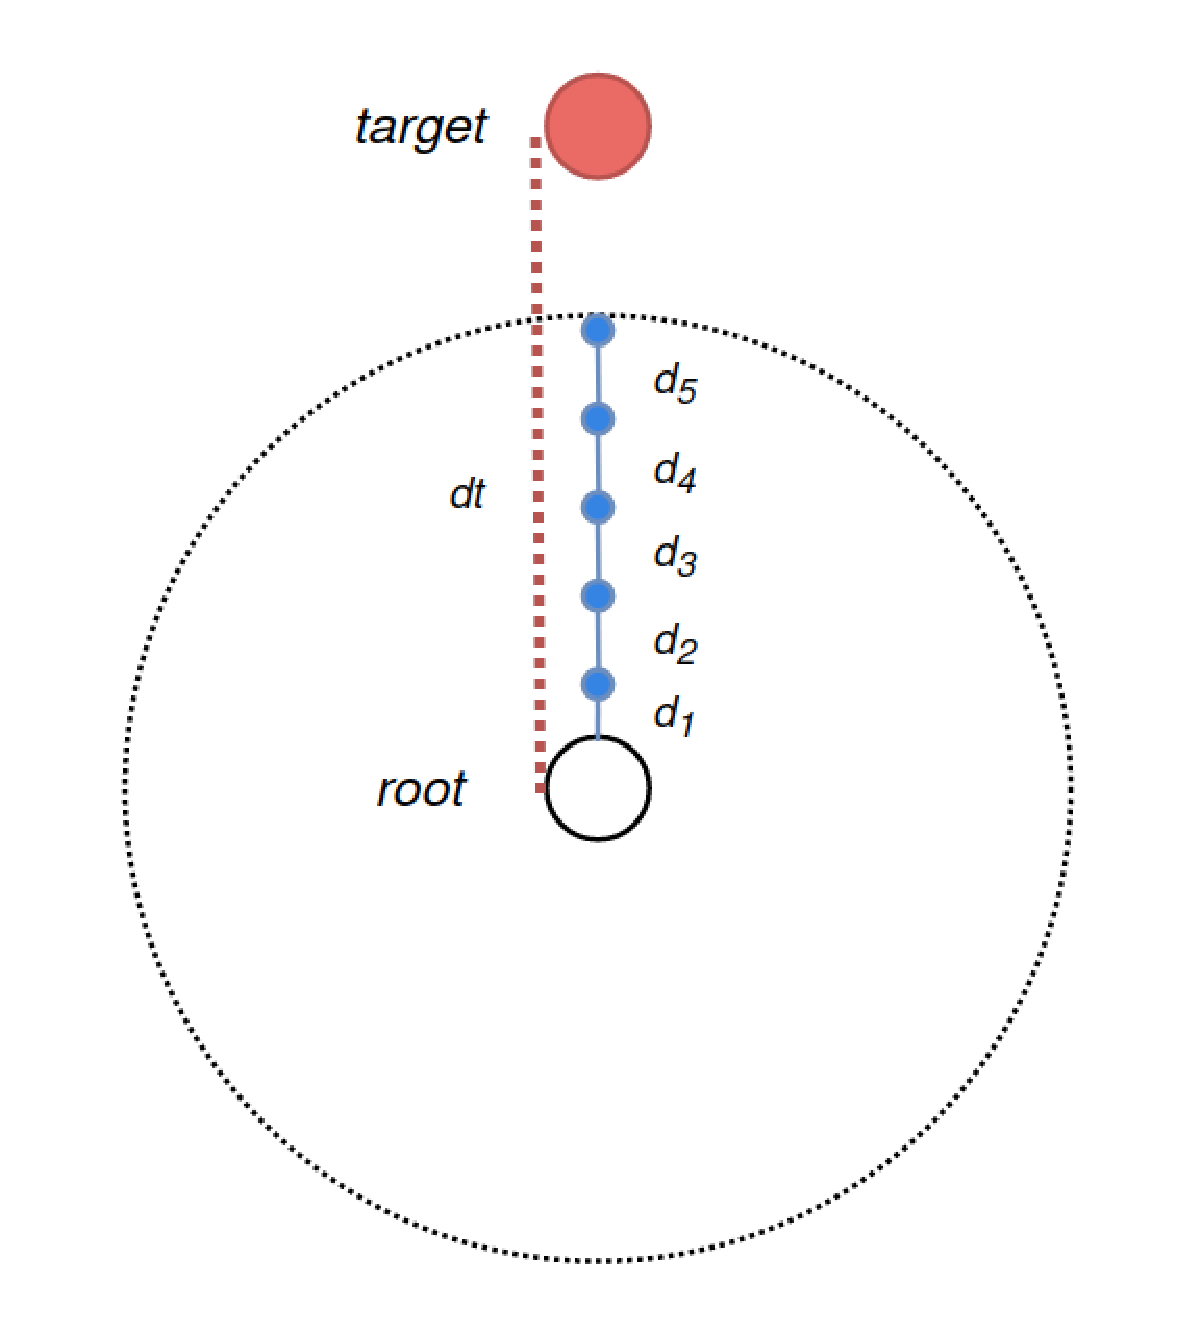
\includegraphics[width=0.5\textwidth]{grafika/unreachable_dist_1.eps}
    \caption{An IK problem with no solution where the target is unreachable
    because the sum of segment distances is less than the distance between the
    root and the target \(\sum_{i=1}^{n}d_i < dt\) }
    \label{fig:unreachable_dist1}
\end{figure}

\begin{figure}
    \centering
    \captionsetup{justification=centering}
    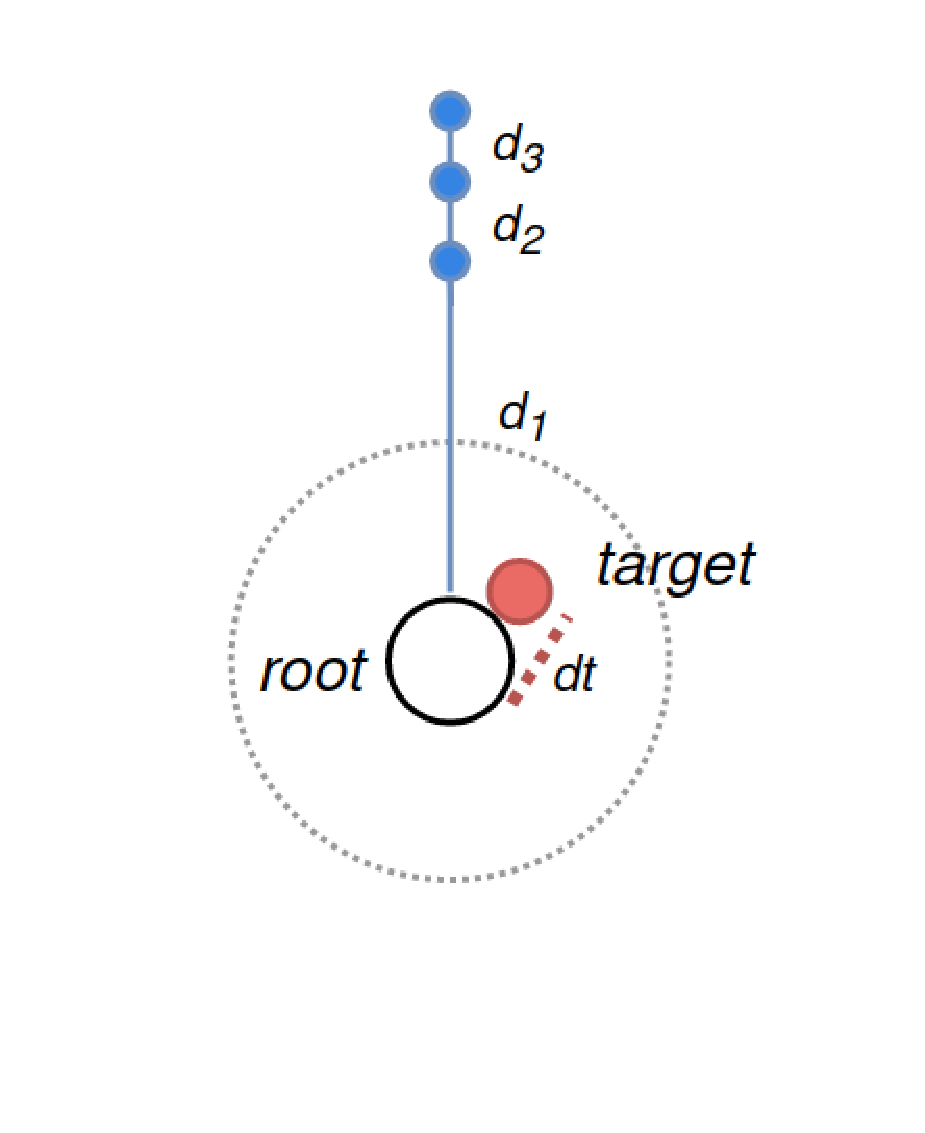
\includegraphics[width=0.4\textwidth]{grafika/unreachable_dist_2.eps}
    \caption{An IK problem with no solution where the target is unreachable
    because the length of the first segment is greater than the summed length of
    the rest of the kinematic chain \(d_1 - \sum_{i=2}^{n}d_i > dt\). This creates
    a radius around the root where if the root's distance to the target is
    smaller than the radius, the target is unreachable.
} \label{fig:unreachable_dist2}
\end{figure}

Another reason for the lack of solutions to an IK problem can be its
over-constraining. Constraints are used to dictate the range of motion of
each joint. For example, they might limit the joint's degrees of freedom by
reducing the dimensions in which it can perform its rotational and translational
transformations. They are often modelled after joints which are present in the
human body, such as hinge joints, ball joints, or pivot joints. A constraint can
also limit the extent of a joint's ability to bend which is defined by the
allowed angle of the joint's rotation in relation to the rotation of its parent
node. If too many of such constraints are added to a kinematic chain, it may
have blind spots for which it is unable to find a configuration of
transformations which can bend the chain to reach the target (Fig.
\ref{fig:unreachable_angles}).

\begin{figure}
    \centering
    \captionsetup{justification=centering}
    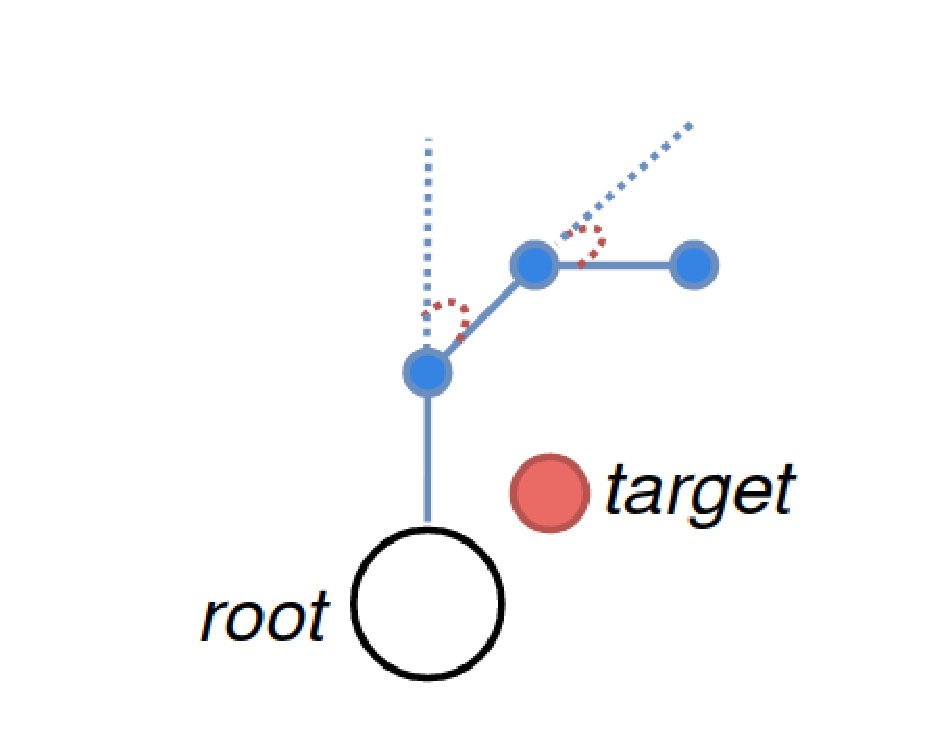
\includegraphics[width=0.4\textwidth]{grafika/unreachable_angles.eps}
    \caption{An IK problem with no solution where the rotational constraints
    placed on the joints prevent the end effector from being able to bend enough
    to reach the target}
    \label{fig:unreachable_angles}
\end{figure}

If a kinematic chain has more than one joint which is classified as an end
effector with its own separate target, a problem with no solutions can be
defined in a way that prevents both end effectors from reaching their target.
If at least one end effector is unable to reach its target then the problem can
be said to be unsolvable. \\

\noindent\textit{One or many solutions}

When an IK problem is not limited by the cases mentioned above, it can have one,
or many solutions depending on the case and constraints. More often the
problem will have multiple solutions, and if the kinematic chain is
unconstrained, the solution set for and IK problem grows very large.

While the introduction of constraints can decrease the number of solutions, the
simplest case to consider for an unconstrained kinematic chain is one where the
chain must stretch to its full extent in order to reach the target. The sum of
the chain's segment lengths \(d_i\) is equal to the distance from the root to
the target \(dt\):
\begin{equation}
    \sum_{i=1}^{n}d_i = dt.
\end{equation}

\section{Underlying principals}
In order to describe the configuration of a given kinematic chain, a set of
scalars \(\theta_1, \dots, \theta_n\) called \textit{joint angles} are defined
for each of the chain's \(n\) joints transforms. A set of \(k\) joint
positions \(\mathbf{s}_1, \dots, \mathbf{s}_k\) is defined for the end
effectors, where these positions are a function of the chain's configuration.
With the joint angles in the form of a column vector \(\bm{\theta} = (\theta_1,
\dots, \theta_n)^T\), and the end effectors as the vector \(\mathbf{s}
= (\mathbf{s}_1, \dots, \mathbf{s}_k)^T\), their relation can be expressed as:
\begin{equation} 
    \mathbf{s} = f(\bm{\theta}).
\end{equation}

The above equation \cite{Aristidou:2018:IK_survey} presents the FK problem where
the position of an end effector is calculated based on the given configuration
of the chain. To define the IK problem, a configuration of scalars must be found
based on the given final positions of the end effectors:
\begin{equation}
    \bm{\theta} = f^{-1}(\mathbf{s}).
\end{equation}

The problem lies in inverting \(f\), as it is non-linear. Taking this into
account, along with the fact that an IK problem may have no solutions, one
solution, or many solutions, an approximation approach can be taken to solve
the problem efficiently. This can be achieved with iterative and heuristic
algorithms.

\section{IK Algorithms}
The methods discussed in this chapter are numerical, which means that
they take an iterative approach to achieve a solution. The numerical methods
can be divided into the \textit{Jacobian}, \textit{Newton}, and
\textit{Heuristic} categories. A comprehensive review of these methods is given
by Aristidou and co-workers in \cite{Aristidou:2018:IK_survey}. For convenience,
the overview of these methods will follow their work.

\subsection{Jacobian methods}
This approach to the IK problem \cite{BALESTRINO19842435, wolovich, Baillieul} offers
a linear approximation through an iterative calculation which estimates a change
to the given configuration of joint scalars necessary to reduce the distance
between an end effector and its desired destination. This is done through the
use of a matrix \(J\) called the Jacobian matrix, which contains partial
derivatives of the entire kinematic chain relative to the set of end effectors.
\(J\) is a \(k \times n\) matrix whose entries are vectors in \(\mathbb{R}^3\),
and it is a function of the chain configuration's joint angle scalars:
\begin{equation}
    J(\bm{\theta})_{ij} = \left(\frac{\partial \mathbf{s}_i}{\partial
    \theta_j}\right)
\end{equation}

\noindent as provided by \cite{rbuss_ik_survey}, where \(n\) and \(k\) are the
previously defined number of joints and number of end effectors in the chain
respectively. Given the position \(\mathbf{p}_j\) of the \(j\)th joint and its
current rotational axis \(\mathbf{v}_j\), each entry of the Jacobian matrix can
be defined by the cross product
\begin{equation}
    \frac{\partial \mathbf{s}_i}{\partial \theta_j} = \mathbf{v}_j \times (\mathbf{s}_i
    - \mathbf{p}_j).
\end{equation}

With prime notation denoting a first derivative with respect to time, the
forward dynamics equation can be written as
\begin{equation}
    \mathbf{s}^\prime = J\bm{\theta}^\prime.
\end{equation}

A change to the kinematic chain's configuration \(\Delta \bm{\theta}\) is then
needed, which when applied, updates the end effectors to minimize their distance
to the targets. The resulting change in the end effector positions \(\Delta
\mathbf{s}\) due to the modification of the configuration is then approximated
as
\begin{equation}
    \Delta \mathbf{s} \approx J \Delta \bm{\theta},
    \label{eqn:fk_approx}
\end{equation}

\noindent and the changes made to the joint scalars should be done in a way
where the change in end effector positions \(\Delta\mathbf{s}\) minimizes the
error \(\mathbf{e}\), which is a vector of changes in position required for each
of the chain's end effectors to reach their desired positions. Supposing that
\(\mathbf{t}_i\) is the target position for the end effector \(i\), the errors
can be defined as \(\mathbf{e}_i = \mathbf{t}_i - \mathbf{s}_i\). By applying a left
matrix multiplication by \(J^{-1}\) to both sides of (\ref{eqn:fk_approx}), the
IK problem for the Jacobian method is rewritten as follows: 
\begin{equation} 
    \Delta \theta \approx J^{-1}\mathbf{e},
\end{equation}
\noindent where \(\Delta\mathbf{s}\) is substituted by \(\mathbf{e}\) due to
them being approximately equal to each other.

A solution to this Jacobian method of the IK problem is not always simple due to
the possibility of a non-invertible matrix, or singularities which prevent
changes of the chain's configurations which achieve the sought-after result in
end effector positions. Certain methods have been brought forward to surmount
these challenges. \\

\noindent\textit{Pseudo-Inverse}

To address the problem of non-invertible Jacobian matrices, the Jacobian
Pseudo-inverse \(J^\dagger\), also called the \textit{Moore-Penrose inverse}
\cite{golub_matrix3} can be used as
a substitute:
\begin{equation}
    \Delta \theta = J^{\dagger}\mathbf{e}.
\end{equation}

The benefit of using the pseudo-inverse method is that the matrix \(J^\dagger\)
is defined for every case of the Jacobian matrix, whether it is invertible or
not. The pseudo-inverse matrix is defined as
\begin{equation}
    J^\dagger = J^T (J J^T)^{-1}.
\end{equation}

Where the pseudo-inverse falls short is when approaching singularities. In these
cases, the resulting values become unstable leading to oscillations. \\

\noindent\textit{Jacobian Transpose}

Another way to overcome the case where \(J\) is a non-invertible matrix is to
use the matrix transpose instead. An so, the inverse is substituted with the
transpose, with a coefficient \(\alpha\):
\begin{equation}
    \Delta \theta = \alpha J^T \mathbf{e}.
\end{equation}

In order to minimize the distance of each \(\mathbf{e}\) between  the end effectors and
their targets, the coefficient \(\alpha\) is calculated with the goal of
achieving the smallest value of \(\mathbf{e}\) after each iteration. The equation
which models this calculation is as follows:

\begin{equation}
    \alpha = \frac
        {
            \langle\mathbf{e}, J J^T \mathbf{e}\rangle
        }
        {
            \langle J J^T \mathbf{e},J J^T \mathbf{e} \rangle
        },
\end{equation}
where the angular brackets represent a dot product operation between the two
values contained inside them. The value of the coefficient \(\alpha\) must be
small enough to avoid oscillations, and due to this the process of converging
end effectors on the targets is slow and requires many iterations to achieve
a desired configuration. \\

\noindent\textit{Other Jacobian methods}

A multitude of approaches to the IK problem using Jacobian methods have been
suggested, some of which are variations or combinations of the presented
methods. Among others, the Singular Value Decomposition method \cite{num_recipes}
extends the pseudo-inverse method with orthogonal matrices, the Damped
Least Squares method \cite{Wampler1986ManipulatorIK} helps avoid problems with
singularities present in the pseudo-inverse method, the Pseudo-inverse Damped
Least Squares method \cite{maciejewski, num_recipes} combines the two previously
mentioned methods to improve their instability when nearing singularities, and
the Selectively Damped Lease Squares method \cite{buss_kim_sdls} builds on the
previous method to converge in fewer iterations and optimize for multiple end
effectors. A deep-learning approach to the Damped Lease Squares method was also
proposed \cite{wang_dldls} with the aim of predicting the most optimal value for
certain coefficients.

\subsection{Newton Methods}
The Newton methods approach IK as a minimization problem, and are based on
a second order Taylor series expansion of \(f(x + \sigma)\):
\begin{equation}
    f(x + \sigma) \approx f(x) + [\nabla f(x)]^T \sigma + \frac{1}{2} \sigma^T
    \nabla^2 f(x) \sigma,
\end{equation}
where \(f(x)\) is the current joint configuration, \(f(x + \sigma)\)
is the desired joint configuration, and \(\sigma\) is the required modification
to \(f(x)\) so that it satisfies \(f(x + \sigma)\). Next, \(\nabla f(x)\) is
the gradient of the objective function, where assuming the notation of the end
effector position as \(e\) and goal position as \(g\), it can be defined as the
Jacobian \(\nabla f(x) = J(e - g)\). Lastly, \(\nabla^2 f(x)\) is the Hessian
matrix, a square matrix of second-order partial derivatives as opposed to the
first-order partial derivatives of the Jacobian matrix. Following the method
described in \cite{nocedal_newton}, the search direction \(p^N_k\) is
\begin{equation}
    p^N_k = [\nabla^2 f(x)]^{-1} \nabla f(x).
\end{equation}

The Newton methods have the advantage over the Jacobian inverse methods in the
smoothness of the movement and the lack of singularity problems, which allows
them to avoid oscillations. The methods also tend to converge
in fewer iterations. However, the complexity of the Hessian matrix drastically
raises the computational costs for each iteration. A few methods have been
brought forward which aim to approximate the Hessian matrix to reduce the
complexity of the problem \cite{fletcher_newton, siciliano_1990,
Chin1997ClosedformAG}, however the computational costs remain relatively high. 

\subsection{Heuristic IK algorithms}
Heuristic algorithms avoid the need for complex equations and heavy
computations, and instead act as techniques to achieve an approximate solution
iteratively in a much more simple way. These methods are very popular in the
domain of computer graphics and animation, due to the problems not needing
extremely accurate solutions but benefiting from a simple and fast approach in
the real-time environment of video games. \\

\noindent\textit{Cyclic Coordinate Descent}

The Cyclic Coordinate Descent (CCD) algorithm \cite{ccd} is one of the simplest and most
used IK solutions in the computer games industry. It also finds
applications in robotics as well as the already mentioned protein structure
prediction \cite{ccd_protein}. 

The algorithm acts on each joint transform separately, minimizing the distance
between the end effector and the target by finding the appropriate angle by
which it should rotate the given joint. The iteration begins at the end of the
chain, excluding the end effector. The desired angle of rotation is calculated by
finding lines, one of which passes through the current joint and the end
effector, while the other passes through the current joint and the target. The
angle between these two lines is the angle by which the current joint should
be rotated in order to place the end effector on the line spanning between the
current joint and the target, thus reducing the distance between the end
effector and the target as much as possible. This process is illustrated in Fig.
\ref{fig:ccd}. The algorithm is repeated iteratively until the distance between the end
effector and the target is smaller than some threshold.

\begin{figure}
    \centering
    \captionsetup{justification=centering}
    \topinset{\bfseries(1)}{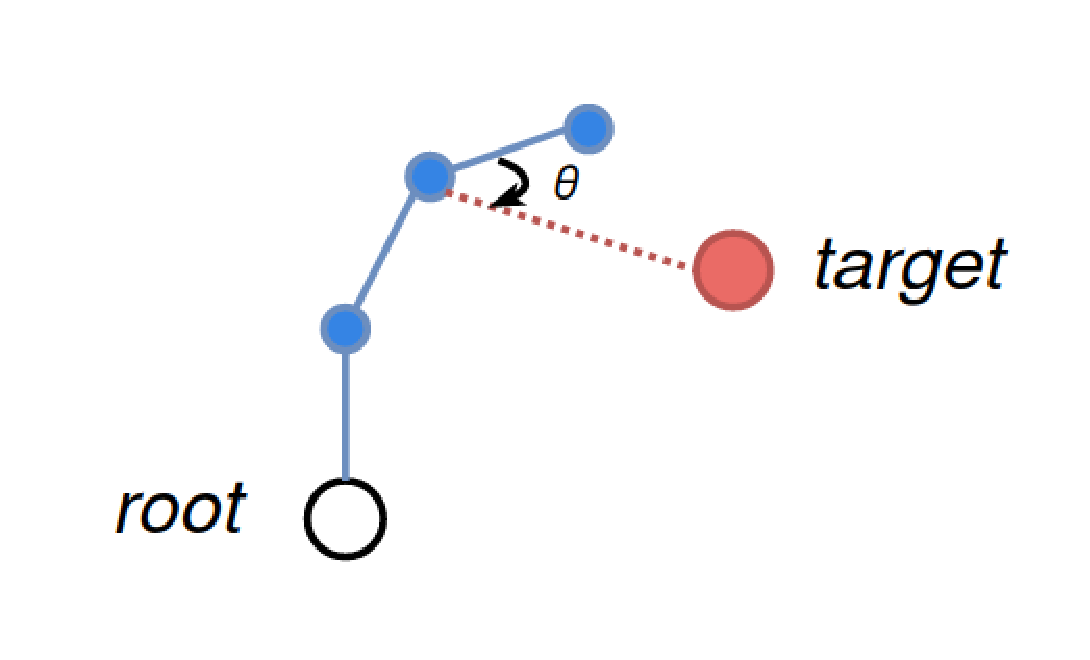
\includegraphics[width=0.4\textwidth]{grafika/ccd_1}}{0.2in}{0.2in}
    \topinset{\bfseries(2)}{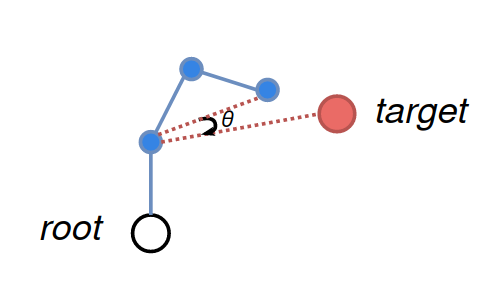
\includegraphics[width=0.4\textwidth]{grafika/ccd_2}}{0.2in}{0.2in}
    \topinset{\bfseries(3)}{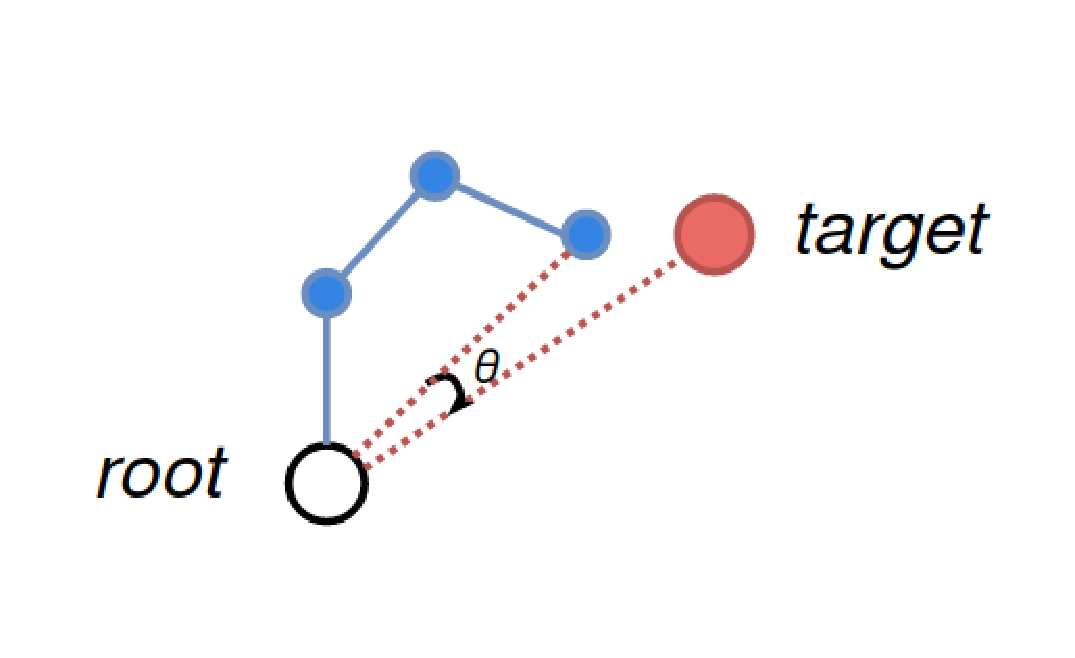
\includegraphics[width=0.4\textwidth]{grafika/ccd_3}}{0.2in}{0.2in}
    \topinset{\bfseries(4)}{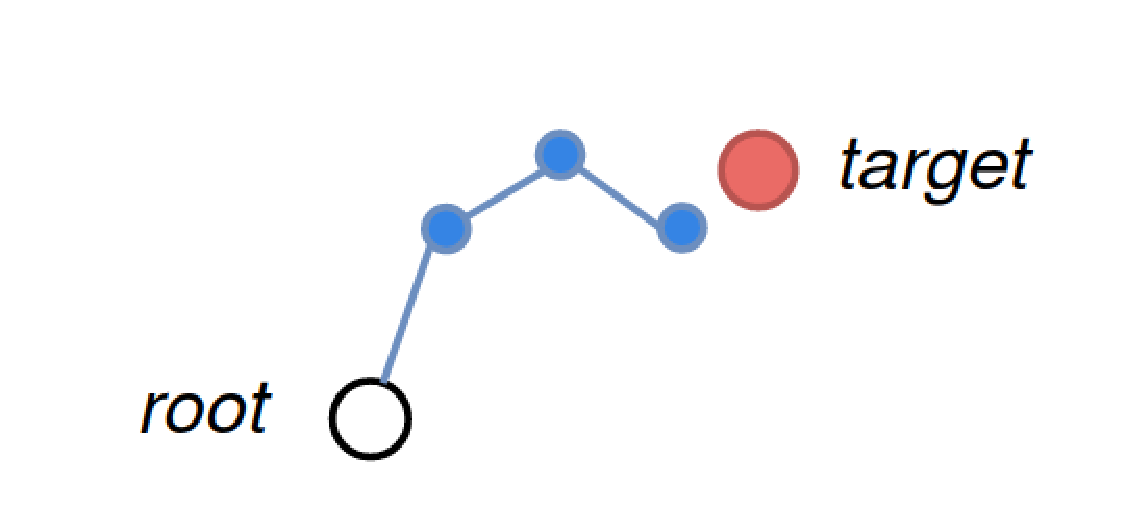
\includegraphics[width=0.4\textwidth]{grafika/ccd_4}}{0.2in}{0.2in}
    \caption{A single pass of the CCD algorithm}
    \label{fig:ccd}
\end{figure}

While the CCD algorithm is very fast and simple to implement, it often produces
unrealistic movements and unnatural poses when applied to a kinematic chain,
partly due to the fact that the joints closer to the end effector have a high
impact on the resolution of the problem, and the joints further away have
a smaller impact. The unequal distribution of adjustments in the chain's
configuration lead to chaotic animations. The algorithm also has a lesser
affinity for solving IK problems with multiple end effectors, and to overcome
this, a system with multiple end effectors must first be broken down into
independent chains. \\

\noindent\textit{Forward and Backward Reaching Inverse Kinematics}

The Forward and Backward Reaching Inverse Kinematics (FABRIK) algorithm
\cite{Aristidou2011} is another heuristic approach to the IK problem which
gained popularity in computer graphics and video games. 

Like the CCD algorithm, FABRIK iterates over the joints of a kinematic chain,
adjusting them one at a time. However, this algorithm involves two passes per
iteration where, as the name suggests, one pass is done starting from the end
effector iterating towards the root, while the second pass is done in a reversed
order as shown in Fig. \ref{fig:fabrik}. The algorithm starts by checking if the
target is in reach before proceeding to iterate over the kinematic chain. 

\begin{figure}
    \centering
    \captionsetup{justification=centering}
    \begin{subfigure}{0.2\textwidth}
        \centering
        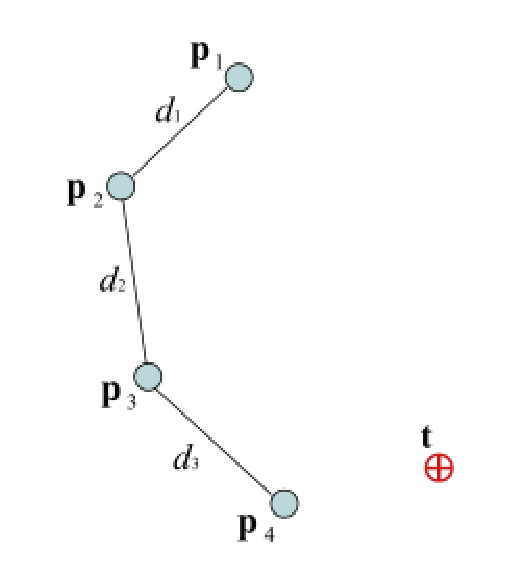
\includegraphics[width=\linewidth]{grafika/fabrik_iteration1.eps}
        \subcaption{}
        \label{fig:fabrik1}
    \end{subfigure}
    \begin{subfigure}{0.2\textwidth}
        \centering
        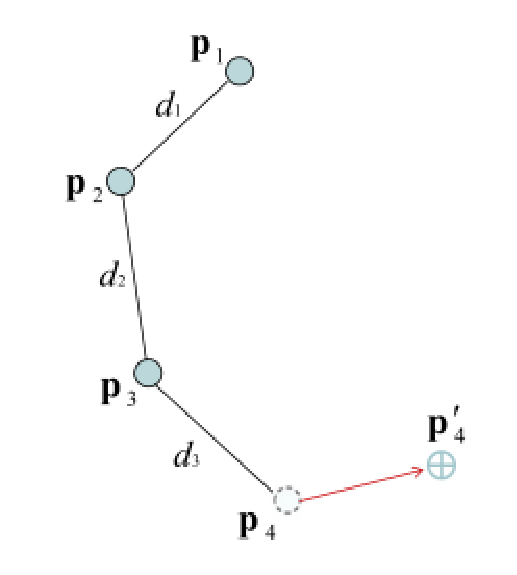
\includegraphics[width=\linewidth]{grafika/fabrik_iteration2.eps}
        \subcaption{}
        \label{fig:fabrik2}
    \end{subfigure}
    \begin{subfigure}{0.2\textwidth}
        \centering
        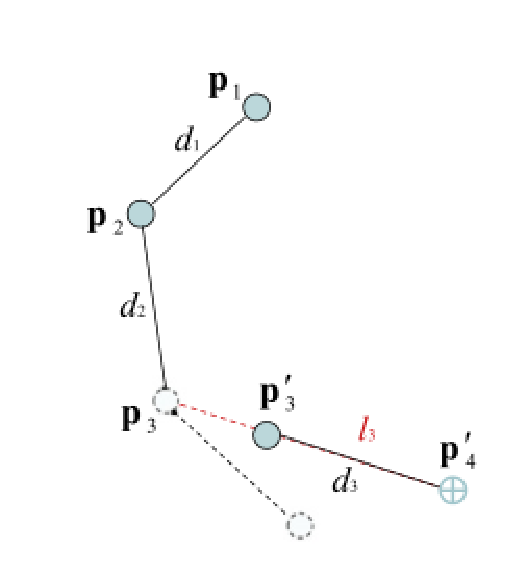
\includegraphics[width=\linewidth]{grafika/fabrik_iteration3.eps}
        \subcaption{}
        \label{fig:fabrik3}
    \end{subfigure}
    \begin{subfigure}{0.2\textwidth}
        \centering
        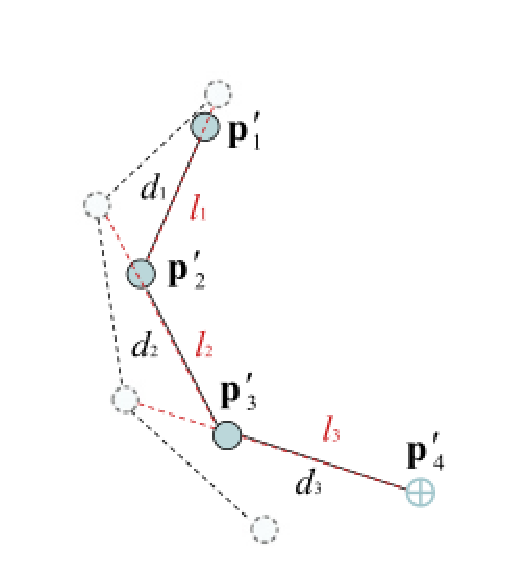
\includegraphics[width=\linewidth]{grafika/fabrik_iteration4.eps}
        \subcaption{}
        \label{fig:fabrik4}
    \end{subfigure}
    \begin{subfigure}{0.2\textwidth}
        \centering
        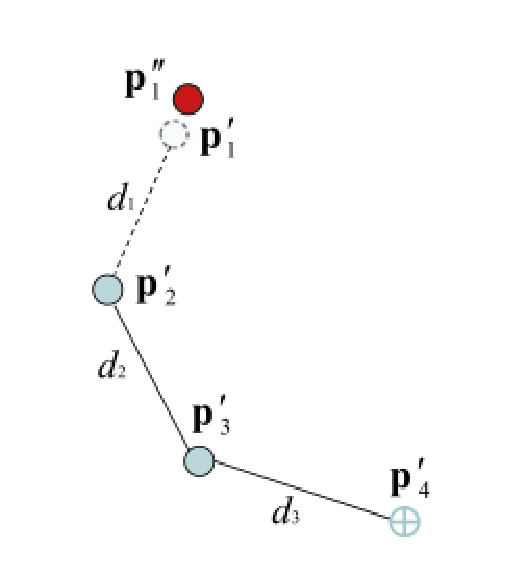
\includegraphics[width=\linewidth]{grafika/fabrik_iteration5.eps}
        \subcaption{}
        \label{fig:fabrik5}
    \end{subfigure}
    \begin{subfigure}{0.2\textwidth}
        \centering
        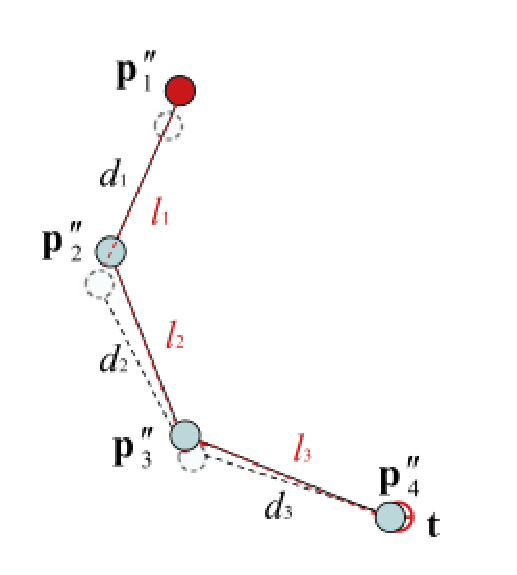
\includegraphics[width=\linewidth]{grafika/fabrik_iteration6.eps}
        \subcaption{}
        \label{fig:fabrik6}
    \end{subfigure}
    \caption{An iteration of the FABRIK algorithm where (a) through (d) are
    detailed steps of the forward pass while (e) and (f) show the solution of
    the backward pass. Source: \cite{Aristidou2011}}
    \label{fig:fabrik}
\end{figure}

% \begin{figure}
%     \centering
%     \captionsetup{justification=centering}
%     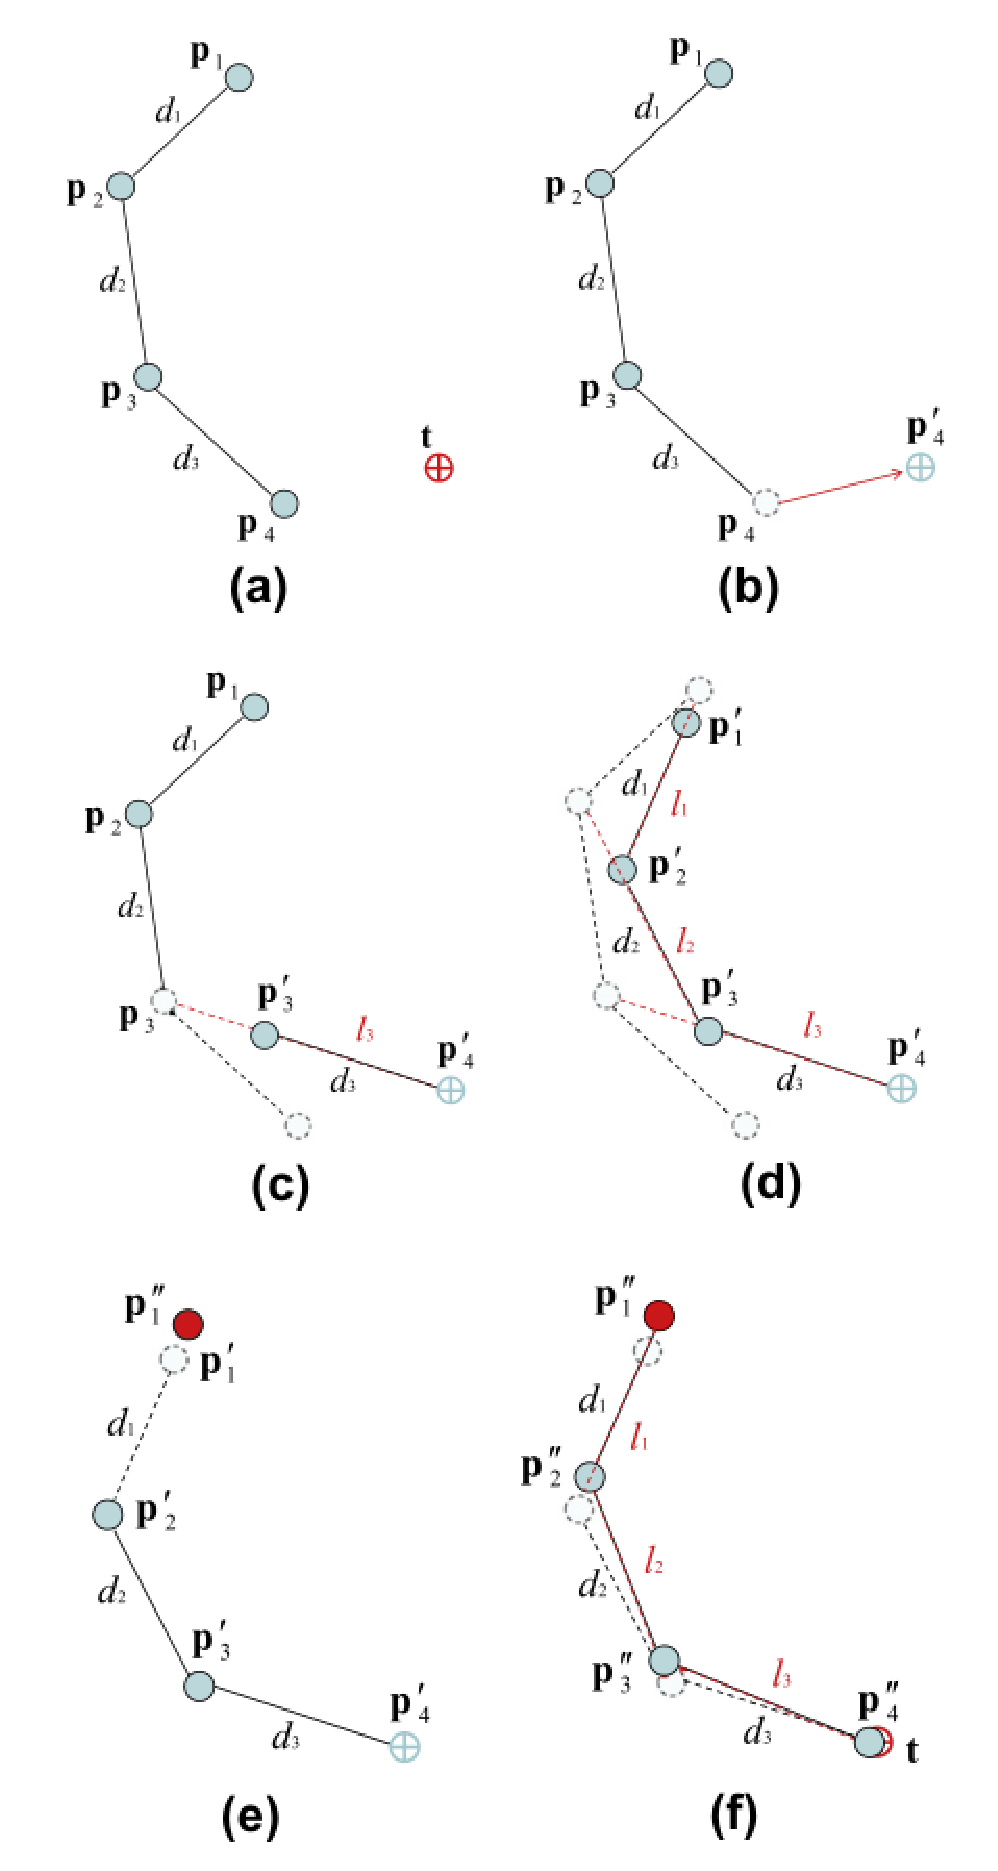
\includegraphics[width=0.4\textwidth]{grafika/fabrik_iteration.eps}
%     \caption{An iteration of the FABRIK algorithm where (a) through (d) are
%     detailed steps of the forward pass while (e) and (f) show the solution of
%     the backward pass. Source: \cite{Aristidou2011}}
%     \label{fig:fabrik}
% \end{figure}

For a set of \(n\) joint positions \(\mathbf{p}_1, \dots, \mathbf{p}_n\) where
\(\mathbf{p}_1\) is the root and \(\mathbf{p}_n\) is the end effector, the forward pass
begins by setting the position of the end effector to that of the target. The
next joint \(\mathbf{p}_{n-1}\) is then linearly interpolated on a line which
passes through its current position and the position of the previously affected
joint, in this case, the end effector. The interpolation is done to preserve the
distance between the joints. Thus, the forward pass of the algorithm can be
modeled by 
\begin{equation}
    \mathbf{p}_i := (1 - \lambda_i)\mathbf{p}_{i+1} + \lambda_i \mathbf{p}_i,
\end{equation}

\noindent where \(\lambda_i\) is a coefficient which ensures that the linear interpolation
preserves the distance between joint positions \(\mathbf{p}_i\) and
\(\mathbf{p}_{i+1}\). When the forward pass is finished, the root ends up being
displaced from its original position, and in order to rectify this a backwards
pass is initiated in a reverse order which starts by setting the root back to
its original position. The iteration proceeds very similarly to the forwards
pass, this time interpolating each joint \(\mathbf{p}_i\) between its current
position and the new position of \(\mathbf{p}_{i-1}\). The backwards pass is then
\begin{equation}
    \mathbf{p}_i := (1 - \lambda_i)\mathbf{p}_{i-1} + \lambda_i \mathbf{p}_i.
\end{equation}

The iterations are repeated until the distance between the end effector and the
target are smaller than some threshold, at which point the problem can be
considered solved.

The FABRIK algorithm is very fast due to its calculations relying on adjusting
positions along a line instead of calculating joint angles. This also majorly
simplifies its implementation. It also provides a more natural configuration as
a solution to the IK problems compared to the CCD algorithm as the degree to
which each joint is adjusted during the iterations is not unevenly distributed
along the chain. Additionally, the FABRIK algorithm is a good fit for computer
graphics and animation because of its ability to handle multiple end effectors
well and to be constrained in multiple ways.

For the purpose of this paper, the FABRIK algorithm was chosen as the
algorithm to be implemented in the demo application. The choice helps avoid the
problems with singularities which exist when using the Jacobian methods, the
complex implementations and heavy calculations of the Newton methods, and
instead provides a fast and lightweight algorithm which is simple to implement
and has a better chance of producing more natural kinematic chain configurations
than the CCD algorithm. The FABRIK algorithm also finds its implementations in
many software programs, including the built-in Unity \textit{Animation Rigging}
package \cite{unity_animation_rigging}.


\chapter{Tools} 
Multiple tools were used in the process of creating the demo application for
this study including the Unity game engine, Blender as a modeling and animation
software, and MakeHuman as a model creation tool. This chapter discusses the
built-in functionalities which make the mentioned tools an effective choice.

\section{MakeHuman}
MakeHuman is an open source tool for making 3D characters. It provides
a convenient way of acquiring a human model which is customizable and can be
exported in various formats in order to be used in other software programs. The
key factors which make this tool suitable for use in the demo application are the
options it provides regarding the complexity of the topology of the model's
mesh, and the choice of skeleton rig. One of the rig presets, which is shown in
Fig. \ref{fig:mh_rig}, is specifically designed to be used for video games. Many
additional cosmetic choices are also offered by the program, allowing for a full
customization of the character. The model is automatically rigged and ready to
be exported and used in an animation software. 

\begin{figure}[!h]
    \centering
    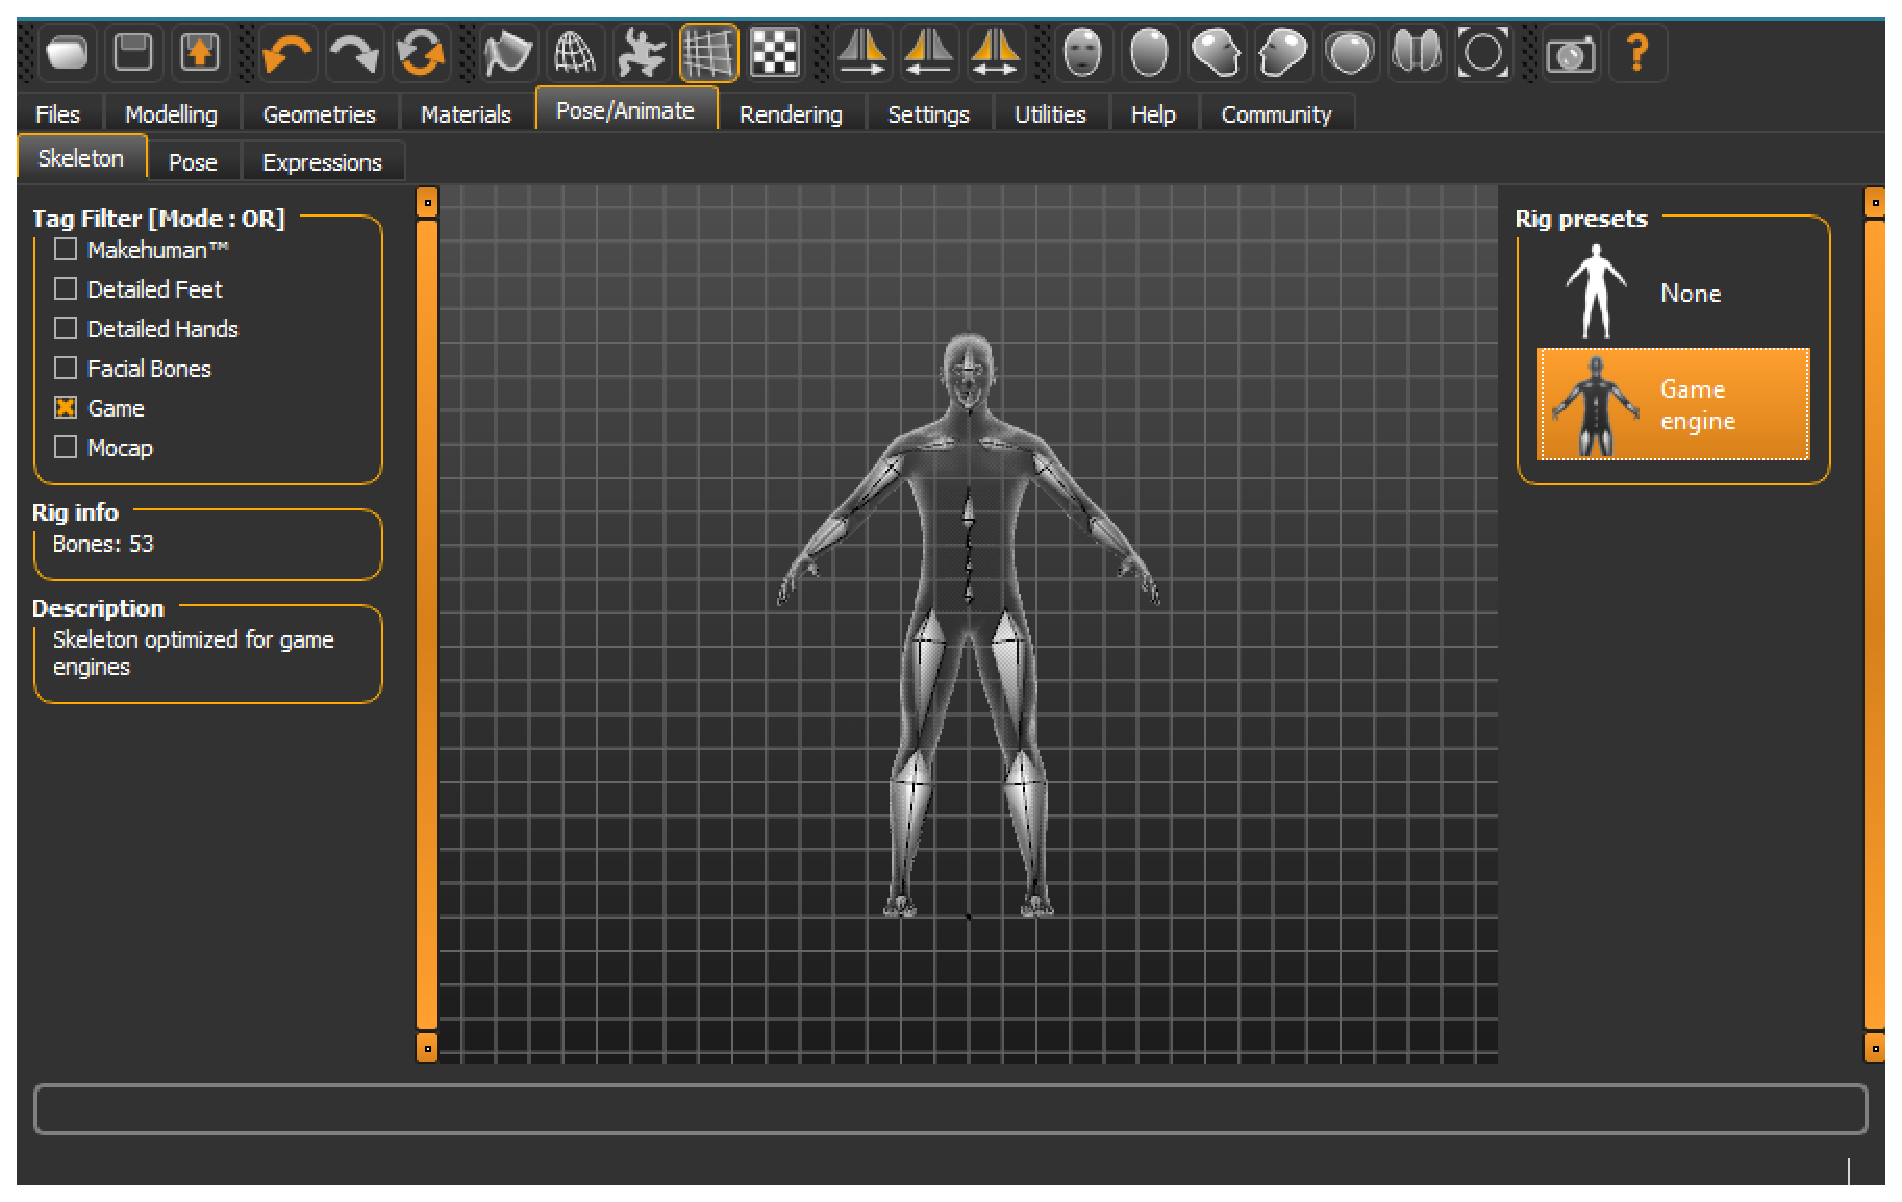
\includegraphics[width=0.9\textwidth]{grafika/make_human_rig.eps}
    \caption{MakeHuman rig selection}
    \label{fig:mh_rig}
\end{figure}

\section{Blender}
The tool for modeling and animation used for the demo application is
Blender. It is a free and open source tool offering a suite of functionalities
including the creation of 3D models, rigging, and animation. 

% The program enables
% users to import models in various formats, which allows the user to use
% externally generated models, such as the ones created in MakeHuman, and animate
% them. 

Blender offers the functionality of importing existing models in various formats
including the \textit{collada} format \cite{collada} which is the default export
option in MakeHuman. Models can also be created from scratch. Blender offers
a 3D modelling tool to create a desired mesh. A custom rig can also be
constructed and attached to the created model. Weights can be painted on the
mesh's vertices for each bone in order to define how much the position of each vertex
depends on the given bone position. 

\begin{figure}[!h]
    \centering
    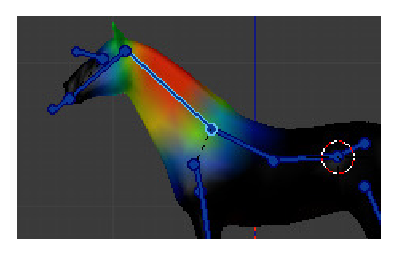
\includegraphics[width=0.4\textwidth]{grafika/weight_paint.eps}
    \caption{Weight painting in Blender. Source: \cite{unity_weights}}
    \label{fig:weights}
\end{figure}

Lastly, an animation sequence can be created for an existing mesh and rig using
the character animation pose editor. The user can define poses for different
points in time by creating key frames on a timeline, and Blender interpolates the
bone positions in between the key frames. This is used to create baked animations
for characters and objects, as well as defining animations that are later
blended with IK procedural animations. An animated model can be exported in the
\textit{fbx} format to be used in other software programs. Unity also supports
importing a model from a \textit{blend} file which is the extension of
a Blender project file. 


\section{Unity}
The Unity game engine is the one tool which was non-negotiable as this work
is meant to specifically focus on the usage of inverse kinematics in said game
engine. Nevertheless, it is a good selection for this use case due to its
advanced 3D support, the built-in packages and functionalities which help
with implementing the techniques discussed in this work, and the overall popularity of
the engine and large community built around it which results in a substantial
amount of documentation and support. 

\subsection{Importing Animations}
Unity enables users to import animated models from external sources using an
\textit{fbx} file or by importing project files from 3D modeling and animation
software such as Blender, Autodesk Maya, Cinema4D, or Autodesk 3ds Max
\cite{unity_import}. However, the modeling software must be installed on the
user's machine in order to import a model from project files, as Unity uses the
programs themselves to unpack the file. 

When importing an animated model into Unity, the import settings allow the user
to break the animation into multiple parts based on start and end times as
demonstrated in Fig. \ref{fig:anim_chunk}. This is convenient, as it allows
multiple animations made in Blender to be placed on a timeline one after the
other as a single animation, which can then be broken up in Unity. It also
allows the user to extract multiple different variations of the same animation,
such as importing the full animation as one whole chunk and also breaking it up
into separate animations for different use cases.

\begin{figure}
    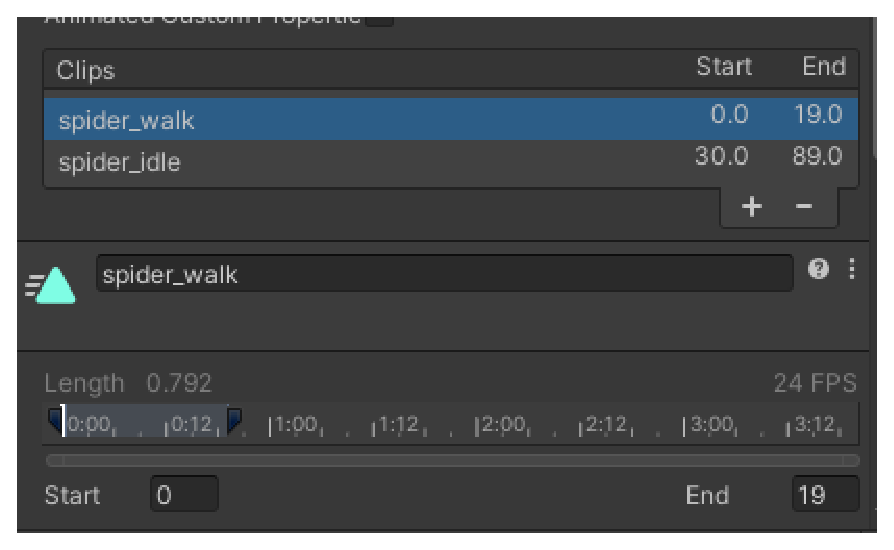
\includegraphics[width=0.5\textwidth]{grafika/animation_chunk_1.eps}
    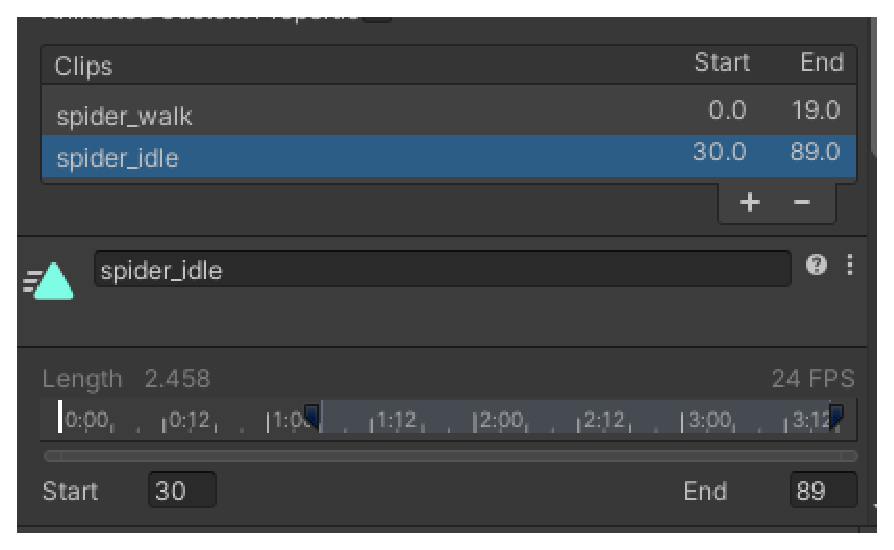
\includegraphics[width=0.5\textwidth]{grafika/animation_chunk_2.eps}
    \caption{Animation clips extracted from a single animation during import}
    \label{fig:anim_chunk}
\end{figure}

\subsection{Animator Controller}
An \textit{Animator controller} allows the user to maintain a set of animation
clips, and the associated transitions which control the flow between each clip
in the form of a state machine as shown in Fig. \ref{fig:anim_state}. Animations must be
added to an \textit{Animator controller} in order to be used by a Unity
\textit{GameObject} \cite{unity_animator}. States can also be controlled
procedurally from scripts by accessing an \textit{Animator} component which must
be attached to the Unity \textit{GameObject} and must hold a reference to the
given \textit{Animator controller}.
 
\begin{figure}
    \centering
    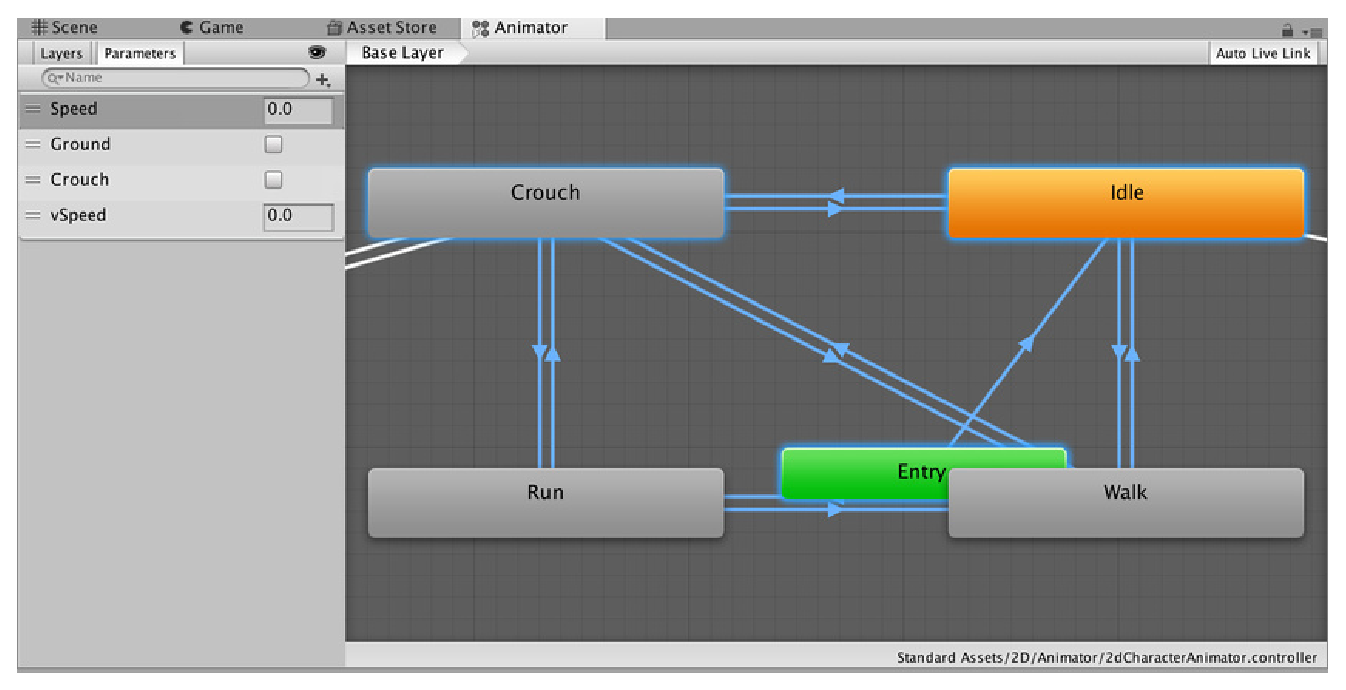
\includegraphics[width=\textwidth]{grafika/animator_controller.eps}
    \caption{Animator controller animation state machine \cite{unity_animator}}
    \label{fig:anim_state}
\end{figure}

The \textit{Animator controller} also has built in IK functionality. This is only
available for humanoid models which have a correctly configured avatar
\cite{unity_ik}. A humanoid avatar is available for models which adhere to a set
of defined general guidelines. In essence, a model which falls into the humanoid
category must have at least 15 bones which are organized in a way which
resembles a human skeleton \cite{unity_humanoid_import}. Humanoid characters
have a few additional functionalities. Namely, because of the criteria required
to qualify as a humanoid model, these models are all similar in structure and as
such, animations can be mapped from one humanoid model to another
\cite{unity_humanoid_avatars}. Additionally, these models have built in
functionality which allows the developer to procedurally control the models IK
weights and positions using the \textit{SetIKPositionWeight,
SetIKRotationWeight, SetIKPosition, SetIKRotation, SetLookAtPosition,
bodyPosition, bodyRotation} functions \cite{unity_ik, unity_humanoid_avatars}.
Because these methods are not available to skeletal structures which do not fit
the humanoid description, they are not applicable to the demo application
created for this paper.

\subsection{Animation Rigging Package}

The Animation Rigging package is available in the Unity Package Manager, and it
provides a much more general approach to the application of inverse kinematics
to skeletal animations. After setting up a rig for a model with an
\textit{Animator} component, a mix of predefined constraints can be added to
enhance the rig, which are briefly described in Table \ref{tbl:ar_constraints}.
The main constraint of interest for this paper is the \textit{Chain IK
Constraint} which implements the FABRIK algorithm. This constraint was useful in
creating a proof of concept for the spider before creating the FABRIK script. It
also provided a good basis for the public interface which such a script should
have to function well in the Unity environment.

\begin{table}
    \centering
    \caption{An available set of predefined constraints from the Animation
    Rigging package which can be applied to a rig
\cite{unity_animation_rigging}.}
    \begin{tabular} { |m{5cm}|m{10cm}| }
        \hline
        Blend Constraint & \footnotesize Allows the constrained object to blend
        between the position and rotation of two other objects. \\
        \hline
        Chain IK Constraint & \footnotesize Applies IK to a hierarchy of objects
        defined by a root and tip. Implements the FABRIK solver. \\
        \hline
        Damped Transform & \footnotesize Damps the position and rotation
        transform values from the source object to the constrained object in
        a hierarchy, increasing in time delay for each next object. \\
        \hline
        Multi-Aim Constraint & \footnotesize Rotates an object to face a chosen
        source object. Can have more than one source object with defined
        weighting. \\
        \hline
        Multi-Parent Constraint & \footnotesize Moves and rotates an object as
        if it is the child of another object in the hierarchy. Does not affect
        scale, and it can have more than one source object with defined
        weighting. \\
        \hline
        Multi-Position Constraint & \footnotesize Moves an object to follow
        a source object. Can have more than one source object with defined
        weighting. \\
        \hline
        Multi-Referential Constraint & \footnotesize Allows an object to act as
        the parent to multiple referenced objects.\\
        \hline
        Multi-Rotation Constraint & \footnotesize Rotates an object to match the
        rotation of its source object. Can have more than one source object with
        defined weighting. \\
        \hline
        Override Transform & \footnotesize Allows a constrained object's
        position and rotation to be overridden in world space, local space, or
        pivot space, by the displacement of the override transform, or by
        precise numerical values. \\
        \hline
        Twist Chain Constraint & \footnotesize Allows controlling world
        rotations on both ends of an object chain hierarchy. The two rotations
        are interpolated along the chain to create a smooth animated hierarchy.
        \\
        \hline
        Twist Correction & \footnotesize Applies a defined percentage of the
        rotation of a source object to chosen twist node objects. \\
        \hline
        Two Bone IK Constraint & \footnotesize Applies IK to a hierarchy
        composed of 2 bones which allows the use of a one target and one hint
        object for control. \\
        \hline

    \end{tabular}
    \label{tbl:ar_constraints}
\end{table}

\chapter{Inverse Kinematics in the Unity Engine} 
The demo application written for the purpose of this work includes two separate
use cases of skeletal animation using inverse kinematics in the Unity engine.
The first example is that of a four legged spider which uses IK as a means to
more naturally adjust its limbs to the terrain it moves around upon. The second
example is the application of inverse kinematics to an animation sequence of
a human character pressing multiple buttons in succession. The use of inverse
kinematics allows the character to adjust its animation to hit all the buttons
without the need for a baked animation targeted towards each button, as well as
dynamically adjust the order of the buttons to be hit. Although there are two
separate use cases demonstrated in this application, both use the same
implementation of the FABRIK algorithm. 


\section{FABRIK implementation}
This implementation of the FABRIK algorithm is based on \cite{Aristidou2011}. For the
purposes of this application, the basic algorithm is implemented without many
additional constraints on the chain's degrees of freedom. The one
constraint added on to this implementation is that of pole targets which will be
further explained when discussing the code behind them.

The script which implements the algorithm in this project takes in a few
parameters required to set up the mechanism which are shown in Fig.
\ref{fig:params}. First and foremost, the root and leaf nodes must be provided
in order to define the kinematic chain which is to be manipulated. The next
object which the script must know is the target transform which the
end effector will attempt to move to. The script must also have a tolerance
parameter which dictates how close the end effector must be to the target for
the position to be considered as solved. All the aforementioned parameters are
required for the script to function. Optionally, a pole target object may be
passed in if the use case requires it to function in a desired manner. 

\begin{figure}
    \centering
    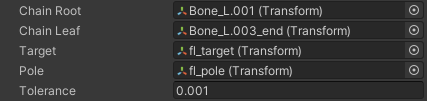
\includegraphics{grafika/parametry_ik.png}
    \caption{FABRIK script parameters}
    \label{fig:params}
\end{figure}

Before any transformations are applied to the joint transforms, their positions
are copied. All operations and calculations are performed on the copied
transforms and at the end of the full pass, the new positions are copied back to
the kinematic chain.

\begin{lstlisting}[basicstyle=\footnotesize, numbers=none,frame=single,
caption={Joint transforms are copied at the start. Operations are performed on
these copied joints, before applying them back to the kinematic
chain},captionpos=b, label=transform_copy, language={[Sharp]c}]
void LateUpdate()
{
    CopyTempPositions();
    ...
    ApplyTempPositions();
}
\end{lstlisting}

The first case which the algorithm must cover is if the distance from the root
to the target object is greater than the sum of distances between each adjacent
bone transform in the defined kinematic chain. In this case, the target is out
of reach. Given that the bones in a skeleton are expected to keep a fixed
length, the end effector will not be able to reach the target, and instead the
kinematic chain straightens and extends in the direction of the target. There is
no need to continue with the iterative portion of the algorithm. A minor
optimization in the implementation is the use of square magnitudes when
comparing distances to avoid the calculation of square roots, thus reducing the
computational costs.

\begin{lstlisting}[basicstyle=\footnotesize, numbers=none,frame=single, caption={Target out of
reach},captionpos=b, label=stretch, language={[Sharp]c}]
void LateUpdate()
{
    ...
    float distRootToTargetSqr = (
        target.position - chainRoot.position
    ).sqrMagnitude;
    if (distRootToTargetSqr > totalDistance * totalDistance)
    {
        StretchToTarget();
    } else {
        ...
    }
    ...
}

void StretchToTarget()
{
    for (var i = 0; i < chainLen; i++)
    {
        float jointDistToTarget = (
            target.position - tempPositions[i]
        ).magnitude;
        var lambda = jointDistances[i] / jointDistToTarget;

        tempPositions[i + 1] =
            (1 - lambda) * tempPositions[i] + lambda * target.position;
    }
}
\end{lstlisting}

If the target is within the reach of the kinematic chain, the iterative process
of forward and backward passes, after which the algorithm is named, is executed.
It is also important to note that the modification of the transforms is done in
Unity's \textit{LateUpdate} function. When using a mix of inverse kinematics and
baked animation, the object to which the IK script is attached will have Unity's
built-in \textit{Animator} component attached as well. If the custom IK script
updates joint transforms in the \textit{Update} method, then their attributes
may be overwritten by the \textit{Animator} component. 


The forward pass of the algorithm iterates through the chain, starting from the
end effector and ending at the root. At the start, the end effector's position
is set to be equal to the position of the target. A vector is then defined which
spans between the end effector and the following joint. This neighbor's position
is then interpolated along the vector so that the original distance between the
two nodes is kept the same. The same operation is performed for each pair of
neighboring nodes throughout the pass. 

\begin{lstlisting}[basicstyle=\footnotesize, numbers=none,frame=single,
caption={FABRIK forward reaching pass},captionpos=b, label=forwards, language={[Sharp]c}]
void ForwardReachingPass()
{
    tempPositions[chainLen] = target.position;
    for (var i = chainLen - 1; i >= 0; i--)
    {
        var dist = (tempPositions[i + 1] - tempPositions[i]).magnitude;
        var lambda = jointDistances[i] / dist;
        tempPositions[i] =
            (1 - lambda) * tempPositions[i + 1]
            + lambda * tempPositions[i];
    }
}
\end{lstlisting}

When the forward pass is complete, the root node is displaced from its original
position. This is undesired, as the root's node position should not be affected
by the algorithm. To remedy this, the next step is to repeat the forwards pass,
but this time in reverse. The root node's position is set equal to what it was
at the beginning of the frame. The next node is then interpolated between its
current position and the root to keep the initial bone length. As with the
forward pass, this is repeated for each subsequent pair of nodes. 

These two steps are repeated cyclically until the end effector is within
a threshold distance of the target. The FABRIK algorithm is a heuristic
algorithm, and as such it does not lead to an exact result. Instead, it aims to
approximate the correct solution and solves the problem in a less complex way.
Again, the square distances are used to avoid the calculation of square roots. 


\begin{lstlisting}[basicstyle=\footnotesize, numbers=none,frame=single,
caption={Main iteration loop of FABRIK},captionpos=b, label=full_loop, language={[Sharp]c}]
void LateUpdate()
{
    ...
    else
    {
        var distEffectorToTargetSqr = (
            tempPositions[chainLen] - target.position
        ).sqrMagnitude;
        while (distEffectorToTargetSqr > tolerance * tolerance)
        {
            ForwardReachingPass();
            BackwardReachingPass();

            distEffectorToTargetSqr = (
                tempPositions[chainLen] - target.position
            ).sqrMagnitude;
        }
        ...
    }
    ...
}
\end{lstlisting}

While the basic FABRIK algorithm allows a kinematic chain adjust so that the end
effector reaches a defined target, the lack of control over this process can
lead to unnatural poses in certain use cases, defeating the purpose of the
procedural animations which are designed to produce a more natural effect. In
order to achieve a higher degree of control in one of the use cases described in
the following section, pole target constraints were implemented as an optional
supplement to the existing algorithm. This approach to the pole target algorithm
is inspired by a video demonstrating this concept \cite{youtube_ik}. 

The pole algorithm acts on every joint in a given kinematic chain excluding the
root and the end effector which already have defined target positions. For each
of the iterated joints \(p[i]\), calculations must take into account the
positions of their preceding joint \(p[i-1]\) and succeeding joint \(p[i+1]\).
A plane is constructed at the position \(p[i-1]\), with a normal vector which
points from \(p[i-1]\) to \(p[i+1]\). Both the pole and the currently
manipulated joint are then projected onto the plane (Fig.
\ref{fig:pole_start}) using Unity plane's \textit{ClosestPointOnPlane} method.
The \textit{Vector3.SignedAngle} method then allows an angle to be found between
both projections by passing the plane's normal vector as the angle axis (Fig.
\ref{fig:pole_projection}). Finally, the current joint's desired position is
calculated by rotating the vector pointing from \(p[i-1]\) to \(p[i]\) around
the plane's normal by the obtained angle, using the
\textit{Quaternion.AngleAxis} method. This can be imagined as lining up the
joint so that its planar projection exists on the line between the origin of the
plane and the pole target's planar projection as demonstrated in Fig.
\ref{fig:pole_end}. The joint keeps its relation to its preceding and succeeding
joints (the angle between vectors pointing from the joint to both surrounding
joints is the same), but it is rotated in order to be positioned as close to the
pole target as possible.

\begin{lstlisting}[basicstyle=\footnotesize, numbers=none,frame=single,
caption={Pole target constraint},captionpos=b, label=poles, language={[Sharp]c}]
void LateUpdate()
{
    ...
        while (distEffectorToTargetSqr > tolerance * tolerance)
        {
            ...
        }
        if (pole != null)
            BendToPole();
    }
    ...
}

void BendToPole()
{
    for (int i = 1; i < chainLen; ++i)
    {
        var plane = new Plane(
            tempPositions[i + 1] - tempPositions[i - 1],
            tempPositions[i - 1]
        );
        var projectedPole = plane.ClosestPointOnPlane((pole.position));
        var projectedBone = plane.ClosestPointOnPlane(
            tempPositions[i]
        );
        var angle = Vector3.SignedAngle(
            projectedBone - tempPositions[i - 1],
            projectedPole - tempPositions[i - 1],
            plane.normal
        );
        tempPositions[i] =
            Quaternion.AngleAxis(angle, plane.normal)
                * (tempPositions[i] - tempPositions[i - 1])
            + tempPositions[i - 1];
    }
}
\end{lstlisting}


\begin{figure}[!h]
    \centering
    \captionsetup{justification=centering}
    \begin{subfigure}{\textwidth}
        \centering
        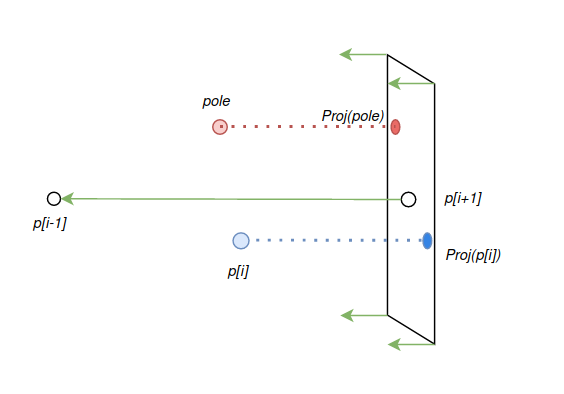
\includegraphics[width=0.6\linewidth]{grafika/pole_start.png}
        \label{fig:pole_start}
    \end{subfigure}
    \begin{subfigure}{\textwidth}
        \centering
        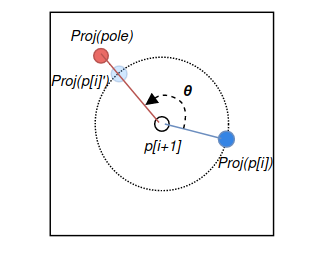
\includegraphics[width=0.4\linewidth]{grafika/pole_projection.png}
        \label{fig:pole_projection}
    \end{subfigure}
    \begin{subfigure}{\textwidth}
        \centering
        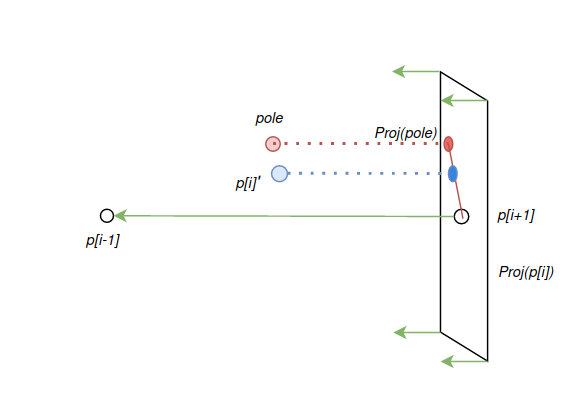
\includegraphics[width=0.6\linewidth]{grafika/pole_end.png}
        \label{fig:pole_end}
    \end{subfigure}
    \caption{A diagram showing the concept behind the implemented pole target
    mechanism. (a) shows the initial setup where a plane is constructed with the
    vector from \textit{p[i+1]} to \textit{p[i-1]} as the normal. Both the
    current joint \textit{p[i]} and the pole target are projected onto the
    plane. (b) is a view of the plane, showing the angle between the
    projections which dictates the new position of the joint \textit{p[i]'}. (c)
    demonstrates the final position of the joint as a result of the pole target
    mechanism.}
    \label{fig:pole_diagram}
\end{figure}

\section{Spider Movement}
The first use case for inverse kinematics in the demo application is that of
a four legged spider. The algorithm is used to adjust the creature's limbs to
uneven terrain, leading to a much more natural and realistic movement. The IK
version of the spider does not have an Animator component, and the whole of the
animation and movement of the spider is done procedurally.
\subsection{Project Setup}
Each one of the spiders legs is treated as a separate kinematic chain. The
spider prefab consists of a container which holds the spider object itself, and
a set of empty objects which the four IK scripts are attached to. The prefab
also contains sets of raycasts and targets. The raycasts serve to scan the
surface of the terrain under the spider, and mark the targets to which each leg
should move.

Raycasts are dispatched from above the spiders legs, and aim in the creatures
local negative Y axis. This ensures that no matter what orientation the spider
finds itself in, the rays are always pointing at the surface which it is
standing on. Masks are applied to the rays, making sure that only terrain
objects are taken into account, while the creature's body itself is not. The ray
cast hit point positions are then applied to each leg's respective target
object. These targets serve as markers for the limbs end effectors. 

\subsection{Scripts}
With the project set up in this manner, scripts must now be added on to make the
scene functional. A script is required for the main movement of the spider, the
raycast logic, and the mechanism which controls the ik targets.

\subsubsection{Raycasts}
The raycast objects contain a script component which dispatches the rays and
sets the appropriate target positions. First, a mask must be established, which
will then be passed into the raycast operation. This is required so that only
terrain is counted as a valid hit. The lack of such a mask may result in
unexpected behavior, such as targets being set on the spider's body itself. The
raycast object is then created, shooting in the local negative Y axis
direction. This ensures that no matter the orientation of the creature, the rays
are sent towards the surface that the spider is standing on. The targets
controlling the spider's legs will not be updating their positions to the
raycast hit points each frame, though their scripts must have knowledge of the
hit positions at any given time. Given this, a separate set of objects are set
to track the raycast hit points each frame.


\subsubsection{Target Logic}
In order for the spider's movement to seem realistic, the targets controlling
each leg must adhere to a set of rules pertaining to their movement. As
mentioned in the raycast section, the IK targets cannot simply be set to track
the raycast hit points. The following is an outline of the rules specified for
the IK targets, which define if it should start moving towards its raycast hit
target:
\begin{itemize}
    \item A target must be grounded to be eligible for a movement sequence.

    \item A target will only begin moving towards the raycast hit point if the
        distance between them is above a specified threshold.

    \item A target is only allowed to begin moving towards the raycast hit
        point if both legs on the opposite diagonal are grounded (See Fig.
        \ref{fig:diagonals}).
\end{itemize}


\begin{figure}
    \centering
    \captionsetup{justification=centering}
    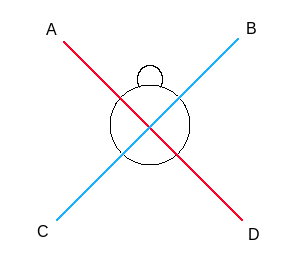
\includegraphics[width=0.4\textwidth]{grafika/diagonals2.png}
    \caption{The diagonals referencing the spiders legs which are used when
    checking if a target is allowed to begin moving, where A and D are on an
opposite diagonal to B and C}
    \label{fig:diagonals}
\end{figure}

When a target satisfies all of these conditions, it makes note of the raycast
hit's current position, which it will use for its upcoming movement sequence.
Once it begins moving, the \textit{Grounded} boolean is set to be false, so that
the other targets know whether they can begin moving or not.

The movement sequence itself is done using Unity's \textit{Vector3.MoveTowards}
method, which takes in a current position vector, a vector to move to, and the
maximum distance to move per frame, which can be used to control the movement
speed. This method allows the target to interpolate its position every frame.
The values fed into this method are simply the target's current position, the
raycast hit target's position, which was recorded right before the beginning of
the movement sequence, and an arbitrary speed value, which is dependent on
\textit{Time.deltaTime} to avoid variations when the frame rate changes. The
only caveat is that in the first half of the movement, the destination vector's
height component is increased with an offset to achieve an arc-like movement.
This produces the effect of lifting the spider's leg.

\begin{lstlisting}[basicstyle=\footnotesize, numbers=none,frame=single,
caption={Execution logic for the legs' movement sequence},captionpos=b,
label=target_move, language={[Sharp]c}]
    float distRemaining = Vector3.Distance(transform.position, _moveTo);
    float heightOffset =
        distRemaining > _totalDist / 2.0f ? heightRise : 0.0f;
    transform.position = Vector3.MoveTowards(
        transform.position,
        new Vector3(_moveTo.x, _moveTo.y + heightOffset, _moveTo.z),
        Time.deltaTime / 0.1f
    );
    if (Vector3.Distance(transform.position, _moveTo) < 0.001f)
        Grounded = true;
\end{lstlisting}

\subsubsection{General Movement}
The main movement script for the IK spider implementation brings the whole
system together. It has three main objectives:

\begin{itemize}

    \item Calculate the rotation of the spider so that it's local up and forward
        vectors can be set accordingly.

    \item React to input by moving the main body of the spider along with the
        raycasts.

    \item Regulate the height of the spiders body above the ground.

\end{itemize}

The first objective - calculating the rotation of the spider - is what allows it
to scale walls and walk upside down on the ceiling. The rotation is determined
based on the limb positions at the beginning of each \textit{Update} call.
First, two vectors are constructed from the end effectors of both sets of
diagonally opposed legs. The local up vector of the spider is then calculated by
taking the cross product of these two vectors. This determines the orientation
of the spider's main body, and it also affects the direction in which the four legs'
rays are cast. The local forward vector is then obtained from the cross product
between the newfound up vector and the spider's right vector. This new vector is
what will be used to determine the direction of movement when the spider
receives input from the user.


\begin{lstlisting}[basicstyle=\footnotesize, numbers=none,frame=single,
caption={Calculating the spider's rotation},captionpos=b, label=rotation, language={[Sharp]c}]
Quaternion calculateRotation()
{
    Vector3 v1 = frLeg.position - blLeg.position;
    Vector3 v2 = flLeg.position - brLeg.position;
    
    _up = Vector3.Cross(v2, v1);
    _forwards = Vector3.Cross(transform.right, _up);
    return Quaternion.LookRotation( _forwards, _up) ;
}
\end{lstlisting}

The second objective - reacting according to input - is quite simple once the
local directional axes are determined. When the script detects a non-zero value
on either the \textit{Horizontal} or \textit{Vertical} axis, it reacts
accordingly by moving the spider along with all the raycast objects. The
\textit{Vertical} axis corresponds to the forward and backward movement of the
spider. The script reacts by simply moving the spider's main body along the
local forward axis mentioned previously. Additionally, the raycasting objects
are offset either forwards or backward depending on the direction of the
movement. This is done because the raycasts must be slightly ahead of the
default leg positions so that the legs end up moving in a natural manner.
The \textit{Horizontal} axis is responsible for rotating the spider about its
local up axis which allows the spider to turn around. 

% \begin{lstlisting}[basicstyle=\footnotesize, numbers=none,frame=single,
% caption={Adjusting the raycast positions so that they are always ahead of the
% spider in the direction in which it is moving. The  variable is the
% input from the  axis.},captionpos=b, label=ray_offset, language={[Sharp]c}]
%     if (Mathf.Abs(yVal) > 0.9f)
%         rays.position = transform.position + _forwards.normalized * yVal * 0.3f + _up.normalized * 1.095f;
% \end{lstlisting}

The second objective - reacting according to input - is quite simple once the
local directional axes are determined. When the script detects a non-zero value
on either the \textit{Horizontal} or \textit{Vertical} axis, it reacts
accordingly by moving the spider along with all the raycast objects. The
\textit{Vertical} axis corresponds to the forward and backward movement of the
spider. The script reacts by simply moving the spider's main body along the
local forward axis mentioned previously. Additionally, the raycasting objects
are offset either forwards or backward depending on the direction of the
movement. This is done because the raycasts must be slightly ahead of the
default leg positions so that the legs end up moving in a natural manner.
The \textit{Horizontal} axis is responsible for rotating the spider about its
local up axis which allows the spider to turn around. 

\begin{lstlisting}[basicstyle=\footnotesize, numbers=none,frame=single,
caption={The raycasts which scan the terrain for leg placement positions are
offset in the direction in which the spider is walking. The \textit{yVal}
variable is the value of the \textit{Vertical} axis input},captionpos=b,
label=ray_offset, language={[Sharp]c}]
    if (Mathf.Abs(yVal) > 0.9f)
        rays.position = transform.position
            + _forwards.normalized * yVal * 0.3f
            + _up.normalized * 1.095f;
\end{lstlisting}

Finally, the spider's height off of the surface must be regulated each frame.
The lack of a gravitational force acting on the body to keep it flush with the
ground, and the unconstrained rotational capability of the creature, means that
the distance between the spider and the surface it is walking on must be
procedurally kept in check. This is done with yet another raycast which
originates from the center of the spider's body and points in the negative up
axis direction. If the distance to the hit point exceeds an acceptable range,
the body is moved towards said range, again using the
\textit{Vector3.MoveTowards} method to linearly interpolate the spiders position
and avoid excessive jerkiness which occurs with a frequent variation in height. 



\section{Human Animation Sequence}
The second example created to demonstrate the use of inverse kinematics for
skeletal animation in Unity is that of a human animation sequence which consists
of pressing multiple buttons in succession. While this may seem like a simple
animation to create in a tool like Blender, such an animation lacks the
adaptability needed for a game which has many differing button pressing
scenarios. The integration of IK into this kind of animation sequence adds the
ability to adjust to multiple amounts of buttons on a panel, different
configurations of button positions, various sequences of buttons to press, and
keeps a consistent hand placement on the buttons without the need to force the
character to stand in one defined position. The example was not made solely
through the use of IK, and instead it uses a mix of baked animations for the
part of the animation which doesn't require variation, and IK for the part of
the animation which should be adaptable.

\subsection{Project Setup}
A human model is exported from the MakeHuman software, imported into Blender for
animation, and then again exported and imported into the Unity engine. The scene
is set up with a group of buttons which are positioned on a wall. The buttons
themselves each have an \textit{EmptyObject} which will provide the transform
needed in order to aim the hand at the given button. The human character is
posted in front of this set up. An Animator component is attached to the human
model in order to make use of certain animations which were extracted from the
full button press animation created in Blender when importing the model into
Unity. Namely, the portions of the animation which consist of raising the hand
to the default pressing position and lowering it back down, are useful in the IK
version of this animation sequence. This is because these two animations are not
dependent on the amount of buttons on the wall, nor the position of the
character relative to the buttons.
\subsection{Scripts}
The whole logic around this animation sequence is done using one script. It must
take in a few public objects as parameters in order to work correctly. Firstly,
the hand's IK target must be passed in to enable the procedural control of the
model's position. The script must also have a reference to the \textit{Rig}
object to which the FABRIK script component is attached to. This is needed in
order to enable and disable the IK depending on the phase of the animation
sequence. When raising and lowering the hand, the baked animations are used and
the IK should be disabled. The next parameter is a list of transforms for each
button to which the IK target will move to in order to achieve the effect of
pressing a button. A couple of private variables are also declared to make the
script functional. These variables hold information such as references to the
animator and FABRIK script components, an idle variable which prevents the
character from starting a new animation sequence before finishing one that was
previously initiated, a value which determines the speed of the hand's movement,
and a list of integers which decide the sequence of buttons to be pressed. One
variable holds the \textit{origin} position which is set to the hand's
position at the moment between the raising of the hand and the press of
a button. This transform is important because it is required in order for the IK
target to know where to return to after it is done pressing a given button. To
be able to set the origin to the appropriate position, a reference to the hand
transform is taken in as the last parameter of the script.

The script's functionality relies on Unity's coroutines \cite{unity_coroutines}.
They enable a method to pause its execution and then continue where it left off
on the next frame. This allows the method to spread a task over multiple frames.
It is useful when chaining together a series of events which must wait for
a previous event to finish its task before beginning its own. The fundamental
part of a coroutine is its \textit{yield} statement which is what pauses the
methods execution. A yield may be used to wait for a certain amount of time, to
wait for a certain boolean expression to evaluate as true, or it can initiate
a nested coroutine and wait for it to end before continuing its own execution.
The yield can also simply return a null value which pauses the execution of the
method until the next frame, which can be useful to spread out a loop to execute
each iteration in a separate frame. In this human animation sequence demo,
nested coroutines are used to enhance readability and maintainability, allowing
for easy reconfiguration of the main loop. 

The first coroutine which is created as a basic building block is the
\textit{HandAnimation} coroutine which takes in an animation name as a string,
executes the animation, and allows the calling function to continue its
execution only after the animation is done. This is possible by checking the
animators state info for the \textit{normalizedTime} attribute. This floating
point value starts at 0 and grows as the animation plays through, with the end
of the animation mapping to a value of 1. The coroutine can therefore yield
a boolean expression checking if the \textit{normalizedTime} value is equal or
greater than one. 

The second building block is the \textit{MoveToTarget} coroutine. This method
takes in a destination vector and a duration. Its purpose is to move the IK
target to a provided destination over a given amount of time. This is
implemented by keeping track of the time elapsed since the beginning of the
coroutine, and then linearly interpolating the position of the target
in a while loop which checks to see if the time elapsed hasn't exceeded the
desired duration of the movement. A \textit{yield return null} in the while loop
ensures that each of its iterations are separated in a way where only one
iteration is executed per frame. A set of two of these coroutines are combined
in the \textit{PressButton} coroutine which combines the movement of the hand
from its origin position to the button, and the movement back to the origin
position.

When the script receives a certain input from the player, and an animation is
not already being played, which is monitored through the \textit{idle} boolean,
then the \textit{PressButtons} coroutine begins execution. This coroutine acts as the
main event loop for the entire animation sequence. The \textit{idle} boolean is
then set to false in order to block the initiation of a subsequent animation
sequence before the current one is finished. The \textit{HandAnimation}
coroutine is executed to play the baked animation of the hand, raising it to its
origin position. The origin position is then saved in the \textit{origin}
variable which will later be used during the IK movements. Now that the baked
animation part of the animation sequence is complete, the IK component of the
rig must be enabled to use its functionality, and have the hand track the IK
target. The \textit{PressButton} coroutine is then executed multiple times in
a loop for every value in the \textit{buttonSequence} array. After the pressing
sequence is complete, the IK component must be disabled before playing the
animation responsible for lowering the character's hand back to its default
position. Lastly, the \textit{idle} boolean can be set back to true as the
current animation sequence is complete and the execution of another animation
should not be blocked.


\chapter{Experiments}
The main purpose of this chapter is to compare animations generated using IK
with baked animations. The comparison is broken up into two categories - visual
quality and performance. 

\section{Baked animations}
 In order to conduct the experiments, a second set of animations were created
 for each of the examples which are shown in the demo application. Below is an
 explanation of the process of creating this second set of animations. \\

\noindent\textit{Spider}

The baked animation version of the spider was animated in Blender. The model
has both idle and walking animations which, in Blender, are placed on
a single timeline, one after the other, as shown in Fig. \ref{fig:timeline}.
Once the model is imported into Unity, the animations can be broken up into
their separate cases, as shown earlier in Chapter 3.3.1 (Fig.
\ref{fig:anim_chunk}). 

\begin{figure}[h!]
    \centering
    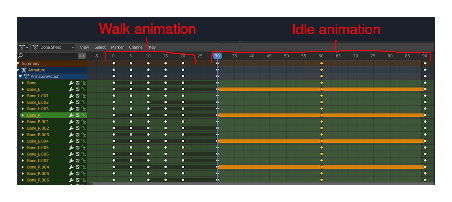
\includegraphics[width=0.7\textwidth]{grafika/blender_timeline.eps}
    \caption{Two animations on a single timeline}
    \label{fig:timeline}
\end{figure}

Once the animations have been imported, a new animation controller is created
for the new spider. The animations are added, this time with the use of a blend
tree (Fig. \ref{fig:s_blendtree}) to, as the name suggests, blend between the
animation smoothly. A third animation state is added to the blend tree
which is the equivalent of the walking animation, but the animation speed is set
to a negative value. This plays the animation in reverse and is used when the
spider is walking backwards. 

\begin{figure}[h!]
    \centering
    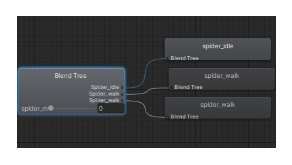
\includegraphics[width=0.7\textwidth]{grafika/spider_blend.eps}
    \caption{Blend tree containing animations for the spider}
    \label{fig:s_blendtree}
\end{figure}

A variable named \textit{spider\_movement} is created in order to control the
animations that are to be played in a given situation, and the manner in which
the transitions should be blended. The thresholds for each animation can be
defined in the blend tree's configuration in the animator (Fig. \ref{fig:s_blendconf}).

\begin{figure}[h!]
    \centering
    \captionsetup{justification=centering}
    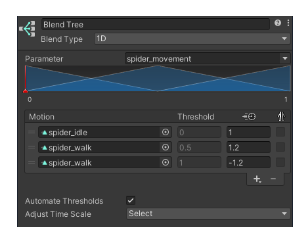
\includegraphics[width=0.7\textwidth]{grafika/spider_blendconf.eps}
    \caption{Configuration of the spider's blend tree which is dependent on
    the \textit{spider\_movement} variable}
    \label{fig:s_blendconf}
\end{figure}

In the spiders movement script, this variable can then be set in reaction to
certain inputs so that the proper animation is activated for each given situation.
To achieve the transition blending, the \textit{spider\_movement} variable
should not be set outright to the value which corresponds to the next animation
state. Instead, the \textit{\_animator.SetFloat} method is used, where the
\textit{\_animator} is a reference to the spider's Animator component. This
method allows the value of \textit{spider\_movement} to be interpolated from the value of
the current animation state to another desired value.
\newline
\begin{lstlisting}[basicstyle=\footnotesize, numbers=none,frame=single,
caption={Transitioning to the spider's idle animation using the
\textit{SetFloat} method},captionpos=b, label=stretch, language={[Sharp]c}]
    if (verticalAxis == 0f && horizontalAxis == 0f)
        _animator.SetFloat("spider_movement", 0f, 0.05f, Time.deltaTime);
\end{lstlisting}

This version of the spider has its movement inspired by the spider from the game
Minecraft, which means that its rotation on the x and z axes is locked. The
spider can rotate about the y-axis when turning to face a different direction,
but it will not adjust to variations in the surface which it walks upon.
Additionally, when the spider encounters a wall, it begins moving
vertically instead of horizontally until it scales the entire obstacle.

\subsubsection{Human}
The baked version of the human character, which performs an animation sequence
consisting of pressing buttons, is animated in Blender. The animation plays one
full sequence of pressing a single button. Chunks of the same animation are used
in the IK version of this animation sequence, described in the previous chapter,
but the baked animation uses the full animation while the IK version uses only
the beginning and the end. However, the animation is still broken up into three
parts when imported into Unity: the raising of the hand, the button pressing
motion, and the lowering of the hand (Fig. \ref{fig:bp_clips}). This is done
because when the character is pressing multiple buttons in a row, the hand
should not be lowered to its starting position after every press.

\begin{figure}[h!]
    \centering
    \captionsetup{justification=centering}
    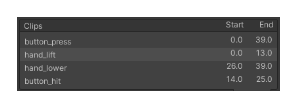
\includegraphics[width=0.7\textwidth]{grafika/bp_clips.eps}
    \caption{The full button press animation is broken up into 3 separate clips}
    \label{fig:bp_clips}
\end{figure}

Another animation controller is created for this version of the human. Unlike
the spider example, the animation states do not have to be blended as they are
all clips which combine to create the full button press animation, and the
transitions are seamless as they are. Because of this, the animation states for
the three animation clips are not part of a blend tree, and instead are just
"floating" states with no defined transitions. The logic for which animation
should be played at what time is defined in the main script attached to the
character. 

The script is a simplified version of the one which controls the IK version of
this character's animation. It has no need for the public parameters present in
it's IK version because there is no IK rig, IK target, or button transforms
which it needs to control. Due to this, there is no list containing the sequence
of buttons to be pressed. It is instead replaced by an integer value which
dictates the number of button presses to execute in one animation sequence in
order to convey the idea that the character is pressing multiple buttons in
a sequence. 

As with the IK version of this script, the logic is based on a set of coroutines
which control the flow of the animation sequence. However, only the
\textit{HandAnimation} coroutine is used as a building block for the sequence
because the whole action is now constructed using baked animations. When the
script receives an input and the animation is not already playing, the sequence
begins by setting the \textit{idle} variable to false in order to prevent the sequence
from being repeated while it is still in progress. All required animation clips
are then set off one after the other, starting with the animation to lift the
hand. This is then followed by the animation clip which is responsible for
hitting the button, and it is repeated in a loop for the number of times defined
by the button press count parameter. Finally, the animation clip for lowering
the hand is executed, and the \textit{idle} boolean is set to true before
terminating the sequence.

\section{Visual Comparison}
The goal of using inverse kinematics to procedurally animate a model in video
games is to achieve a more natural interaction between a character and the
environment. The realism of the interaction is conveyed through how it looks,
and how the animation is a more realistic representation of how such an action
might look in real life. Therefore, the visual integrity of the IK animation as
it adapts to a plethora of scenarios is what sets it apart from a classic
approach through baked animations. 

The walking animation, or any basic movement animation, is the core of what
most characters will be displaying a majority of the time. That being the case,
a natural movement animation will contribute the most to the overall look and
feel of the character. This difference can be clearly noticed by comparing the
two version of the spider implemented in the demo application created for the
purpose of this paper. 

Starting with the idle position, both models look quite natural standing on
a flat surface, as seen in Fig. \ref{fig:sp_flat}.


\begin{figure}[h!]
    \centering
    \captionsetup{justification=centering}
    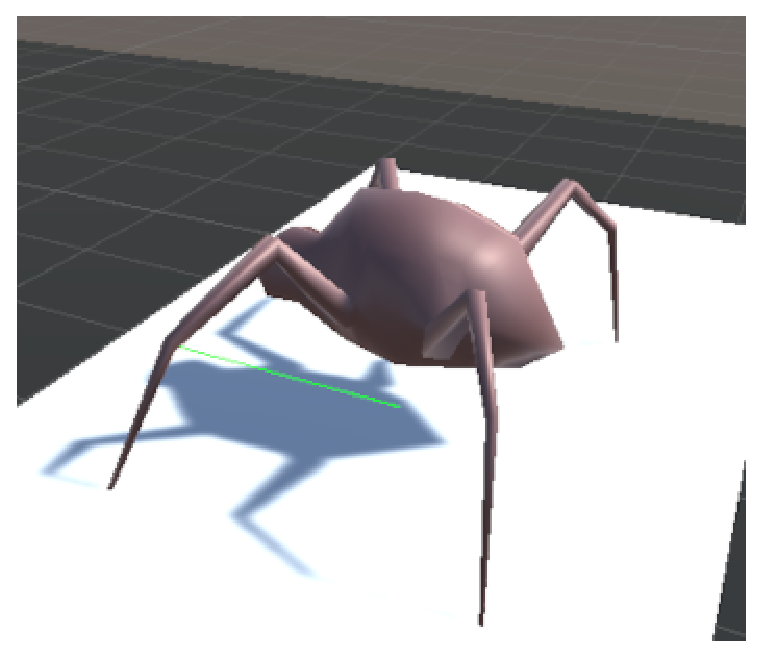
\includegraphics[width=0.4\textwidth]{grafika/sp_b_flat.eps}
    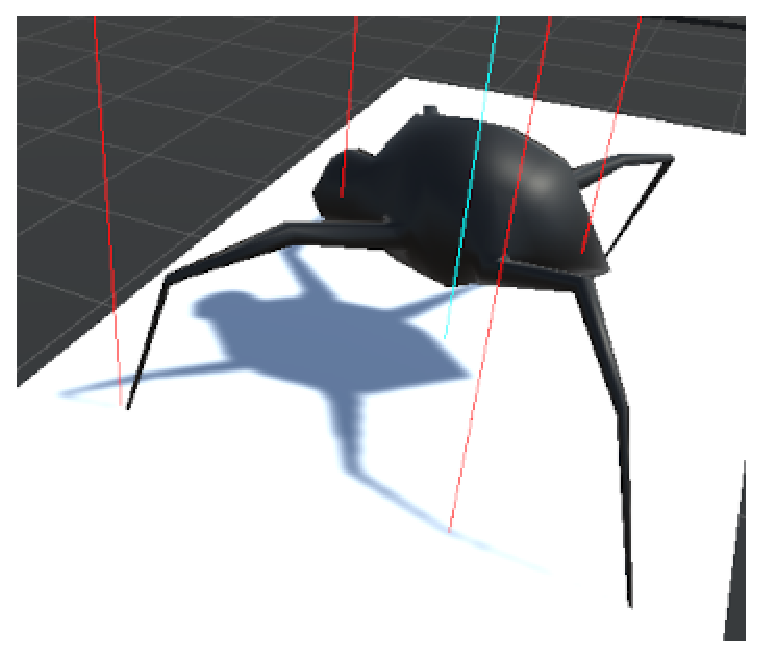
\includegraphics[width=0.4\textwidth]{grafika/sp_ik_flat.eps}
    \caption{A comparison of both models standing on a flat surface}
    \label{fig:sp_flat}
\end{figure}

However, this changes when the surface is uneven. The IK acting on
the legs of the spider on the right in Fig. \ref{fig:sp_round} is able to use
its ray casts to match the surface exactly, while the baked version of the
spider (left) doesn't have this mechanism, and its legs can be seen floating in
the air. The same effect is observed when the spider is moving. The baked
version's legs float when it is moving over uneven or slanted surfaces, which
makes it seem as if the spider was swimming through the air. 

\begin{figure}[h!]
    \centering
    \captionsetup{justification=centering}
    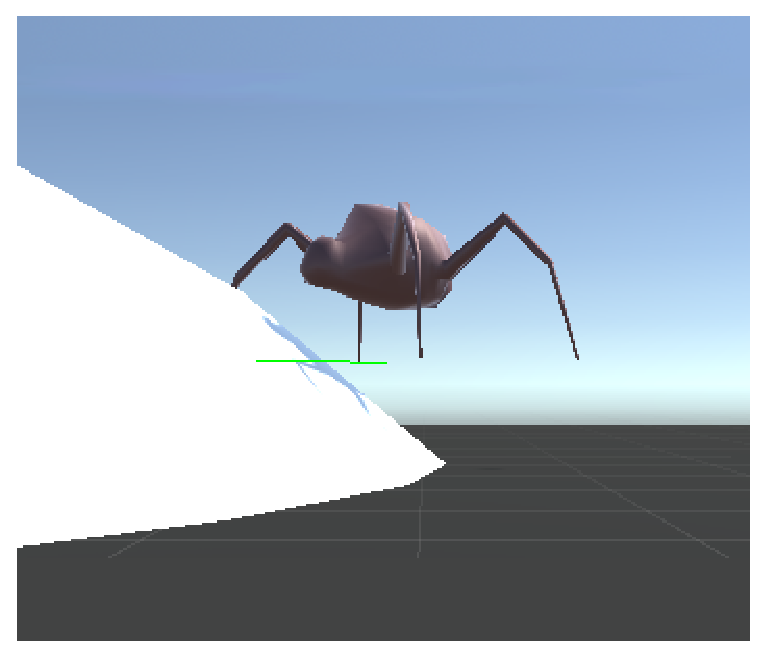
\includegraphics[width=0.4\textwidth]{grafika/sp_b_round.eps}
    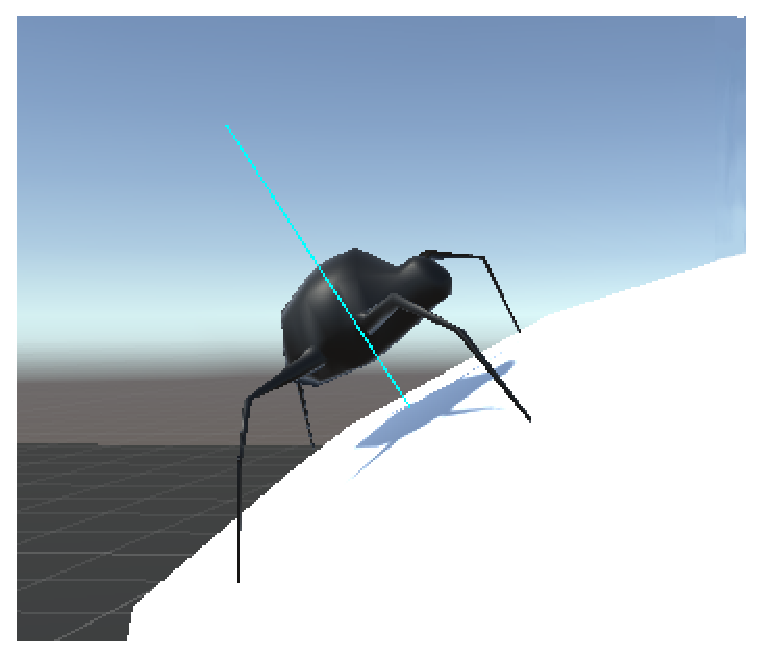
\includegraphics[width=0.4\textwidth]{grafika/sp_ik_round.eps}
    \caption{A comparison of both models standing on an uneven surface}
    \label{fig:sp_round}
\end{figure}

Another difference between the two spiders is how they climb walls. Whereas the
IK version is able to treat it the same as any other surface, the baked version
keeps does not adjust its rotation, and instead climbs the wall head on (Fig.
\ref{fig:sp_wall}). This kind of rotation could have been implemented, however,
the transition between floor and wall would be very unnatural either way and so
an implementation inspired by the spiders in the game Minecraft was used
instead.

\begin{figure}[h!]
    \centering
    \captionsetup{justification=centering}
    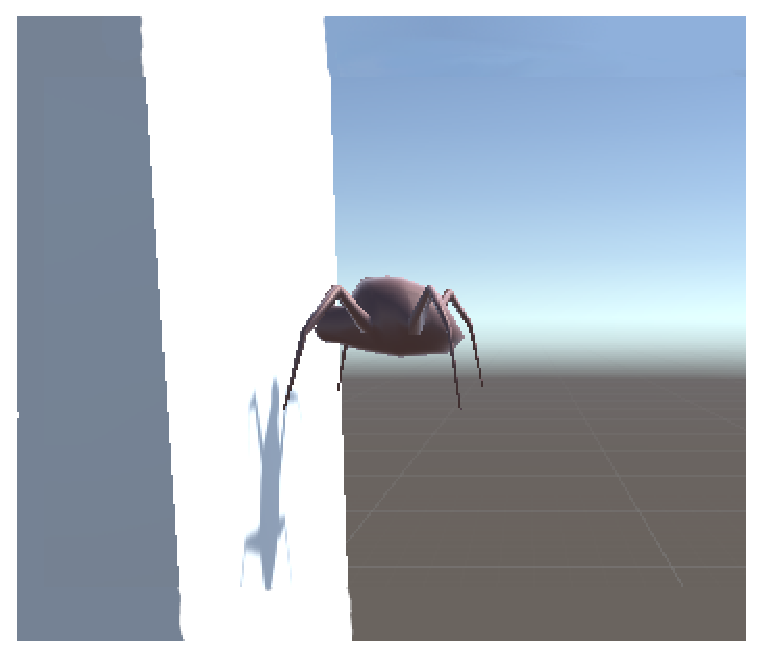
\includegraphics[width=0.4\textwidth]{grafika/sp_b_wall.eps}
    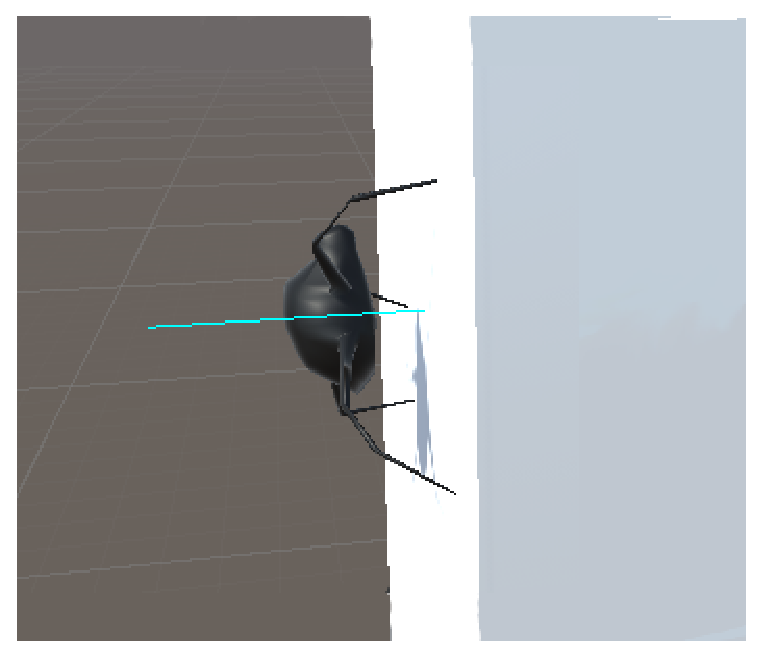
\includegraphics[width=0.4\textwidth]{grafika/sp_ik_wall.eps}
    \caption{A comparison of both models scaling a wall}
    \label{fig:sp_wall}
\end{figure}

One important aspect to note when comparing the realism of both animations is
how the legs move relative to the surface on which they stand. In the case of
the procedural animation, the IK targets controlling the spider's legs remain
fixed in one place until a leg movement is initiated. As a result, no matter the
speed at which the spider is moving, the give the impression that they are
placed on the floor and push away realistically. On the contrary, the baked
animation is played at a certain speed, and it is very hard to match the
animation speed to the spider's movement speed so that the legs seem to stay in a fixed
position on the ground while the spider is moving. This breaks the illusion of
the legs pushing the spider forwards, as they instead glide on the surface out
of sync.

In certain games, the accuracy of animation sequences creates a greater
immersion for the player. In the event that the sequence of pressed buttons is
important, such as a player needing to provide a specific input to hack a code
to open a door, the realism of the game can be elevated through the use of
inverse kinematics. The adaptability of a character's actions can be seen in this
comparison between the baked and IK versions of the button press animation.

When the character is only required to press a single button, while also having
a proper position and orientation relative to the button, the baked animation
looks quite natural, and looks no different from the IK version as shown in Fig.
\ref{fig:h_single}.

\begin{figure}[h!]
    \centering
    \captionsetup{justification=centering}
    \begin{subfigure}{0.4\textwidth}
        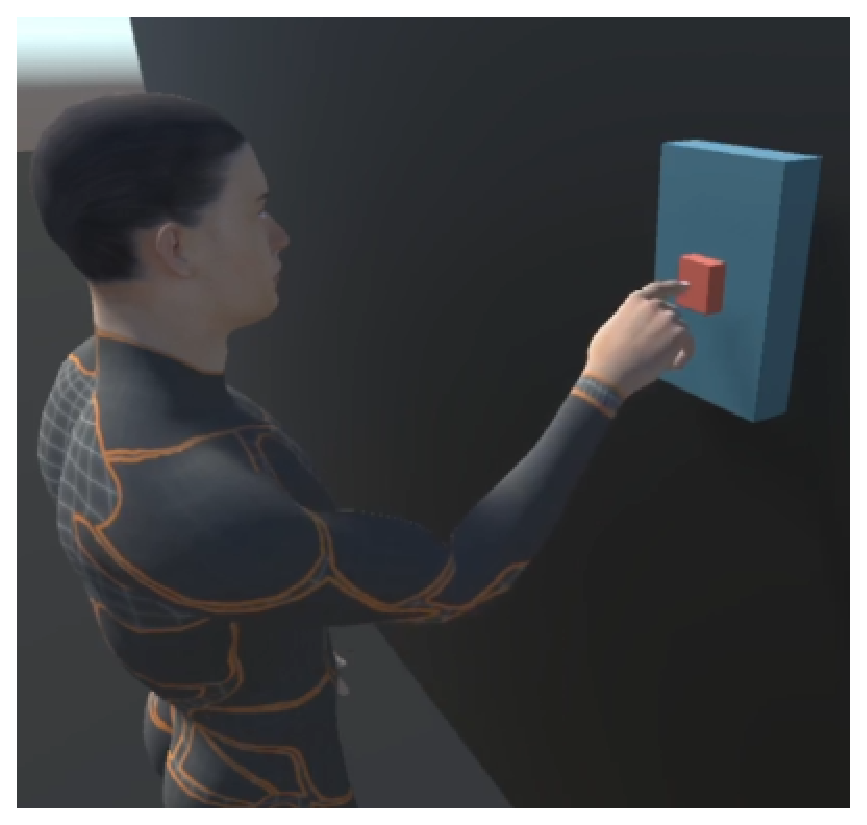
\includegraphics[width=\linewidth]{grafika/h_b_single.eps}
    \end{subfigure}
    \begin{subfigure}{0.4\textwidth}
        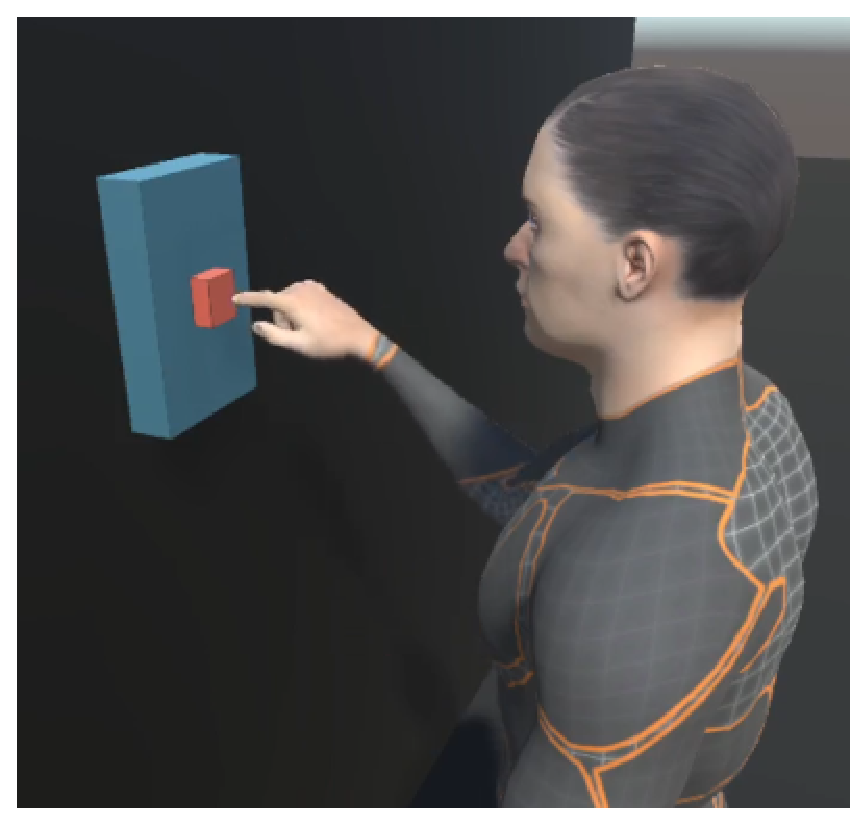
\includegraphics[width=\linewidth]{grafika/h_ik_single.eps}
    \end{subfigure}
    \caption{A comparison of both models pressing a single button. (a) is the
    baked animation and (b) is the IK animation.}
    \label{fig:h_single}
\end{figure}

The difference starts to be noticeable when the character is offset or rotated
from the default position. While the IK target leads the hand correctly to the
button (Fig. \ref{fig:h_ik_offset}), the baked animation has no knowledge of
the characters surroundings, and misses its mark (Fig. \ref{fig:h_b_offset}).
Due to this, for realism to be preserved when using a baked animation, either
the character must be reoriented as part of the action, or a cutscene should be
played for the duration of the action. 

\begin{figure}[h!]
    \centering
    \captionsetup{justification=centering}
    \begin{subfigure}{0.4\textwidth}
        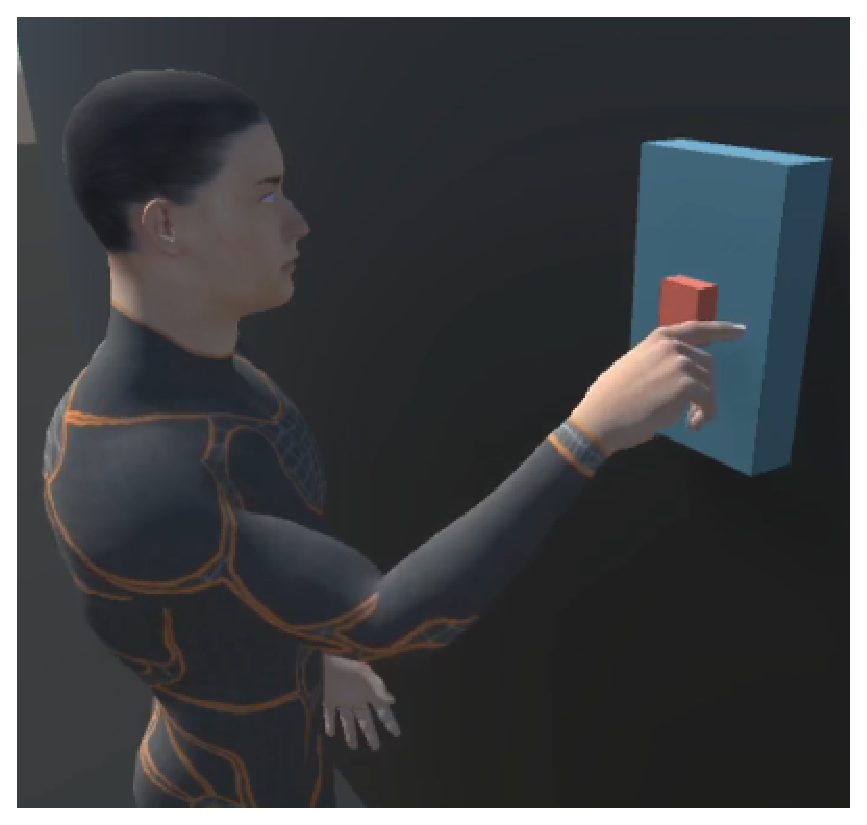
\includegraphics[width=\linewidth]{grafika/h_b_offset.eps}
        \subcaption{Baked animation}
        \label{fig:h_b_offset}
    \end{subfigure}
    \begin{subfigure}{0.4\textwidth}
        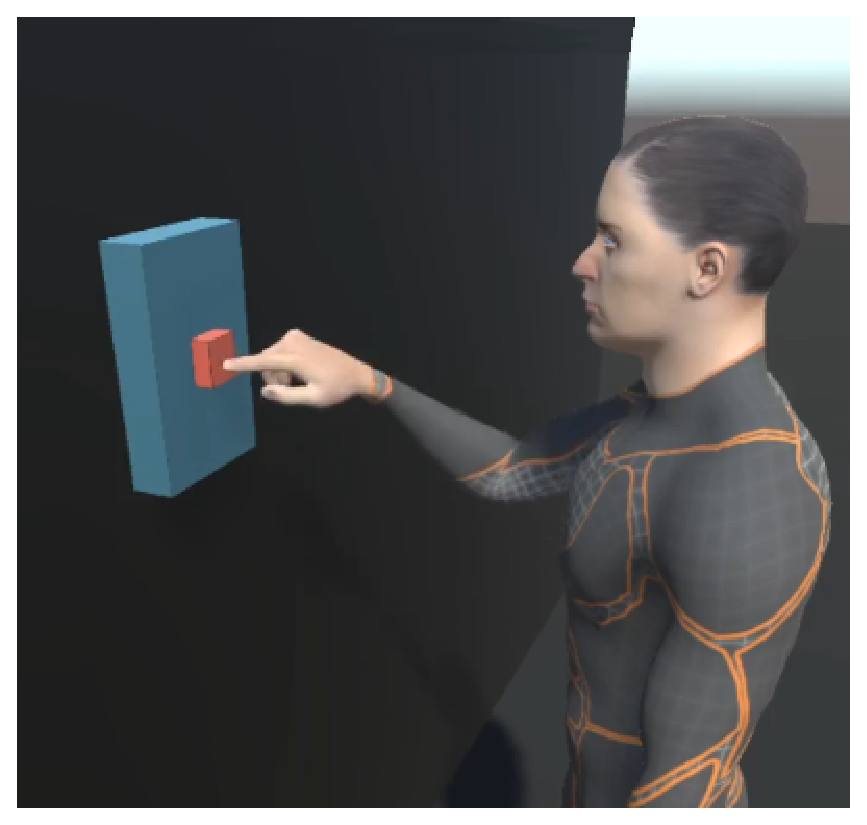
\includegraphics[width=\linewidth]{grafika/h_ik_offset.eps}
        \subcaption{IK animation}
        \label{fig:h_ik_offset}
    \end{subfigure}
    \caption{A comparison of both models pressing a single button after
    offsetting the position and rotation of the characters}
    \label{fig:h_offset}
\end{figure}

The next benefit of the procedural animation is its ability to adapt to a panel
with multiple buttons. The character which is using the baked animation is only
able to aim its hand at one specific point, consequently missing all the
buttons. In the case of a sequence of buttons being pressed, the character
repeats the press in a single spot which doesn't realistically convey the
pressing of a sequence of buttons. This can be slightly improved by constructing
the animation to aim at different buttons on the panel in a generic order. The
downside of this approach is that it falls apart if there is a change in the
amount of buttons, or their positions and configuration. 

Comparing this to the IK animation, as seen in Fig. \ref{fig:h_ik_multiple},
the IK target leads the hand to the appropriate position for each separate
button. This allows for a specific sequence of buttons - taking the door hacking
example from before this would be a player's input - to be pressed in a way
which visually conveys the exact action which was commanded, in a responsive
manner.

\begin{figure}[h!]
    \centering
    \captionsetup{justification=centering}
    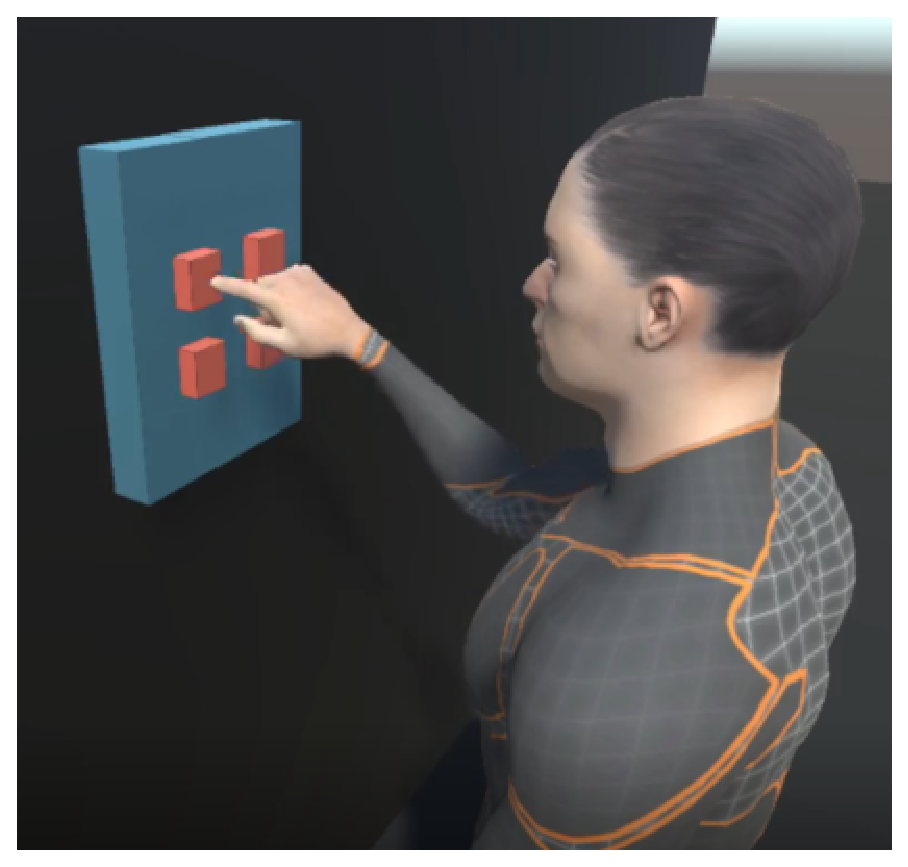
\includegraphics[width=0.4\textwidth]{grafika/h_ik_1.eps}
    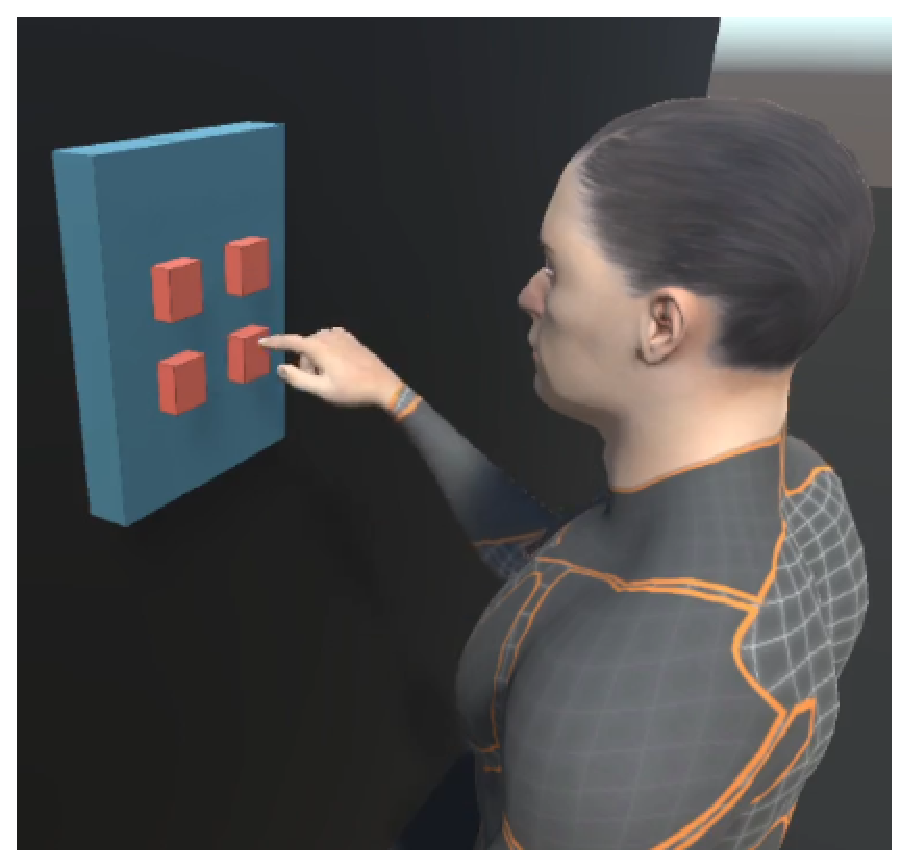
\includegraphics[width=0.4\textwidth]{grafika/h_ik_2.eps}
    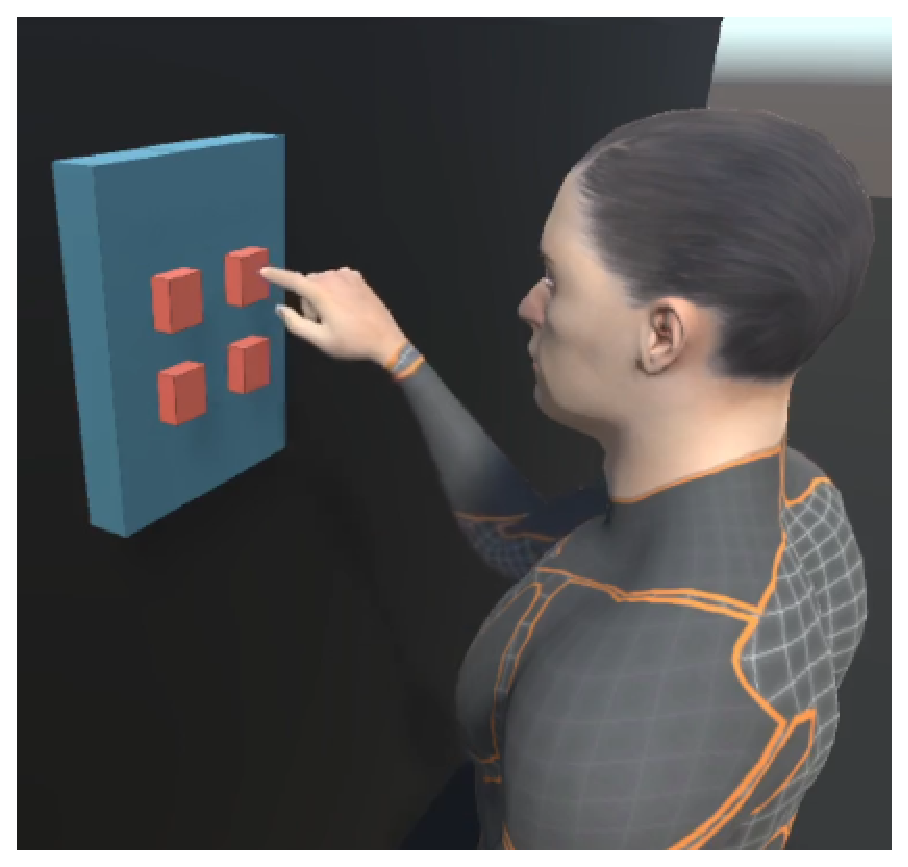
\includegraphics[width=0.4\textwidth]{grafika/h_ik_3.eps}
    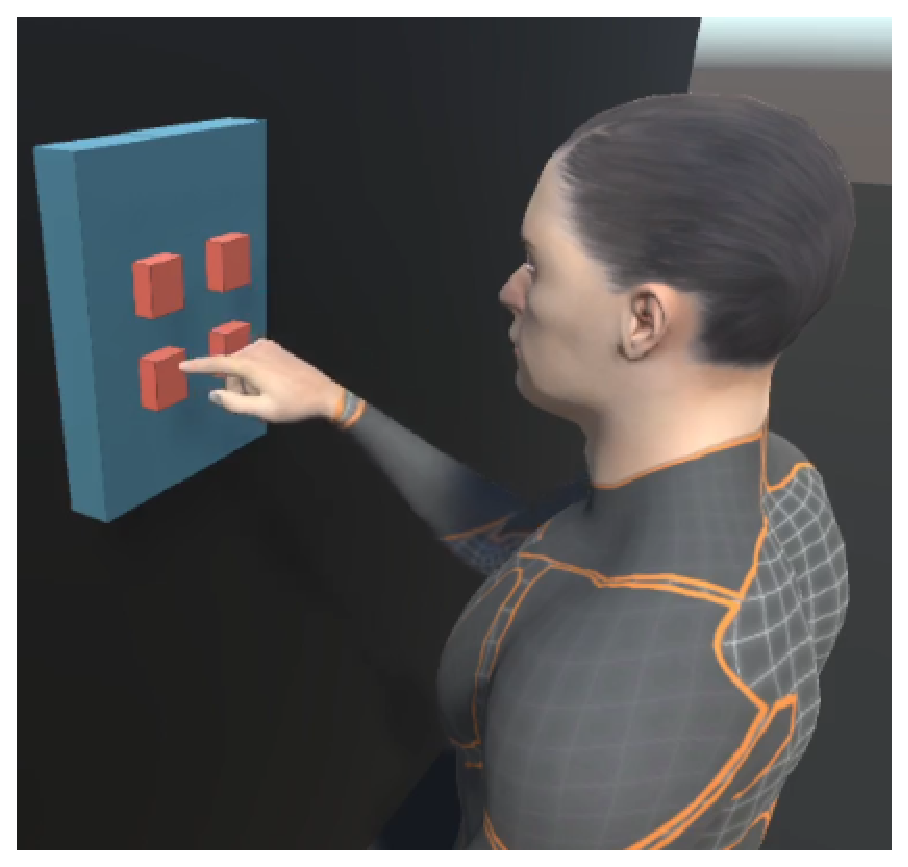
\includegraphics[width=0.4\textwidth]{grafika/h_ik_4.eps}
    \caption{The IK model pressing each of the four buttons on a panel}
    \label{fig:h_ik_multiple}
\end{figure}



\section{Performance Comparison}
One thing to consider when implementing a task procedurally is the
effect it may have on the performance of the application. Resorting to the use
of code and calculations instead of executing a predefined sequence introduces
the potential of increasing the CPU usage and decreasing performance. An
analysis was conducted on the examples created in the demo application using the
Unity Profiler \cite{unity_profiler}. Each experiment was carried out by
spawning 100 objects of each type and comparing the CPU usages both while they
were idle and while they were moving. Some usage categories were discarded as
they were not relevant to the analysis (Fig. \ref{fig:profiler_settings}).

\begin{figure}[h!]
    \centering
    \captionsetup{justification=centering}
    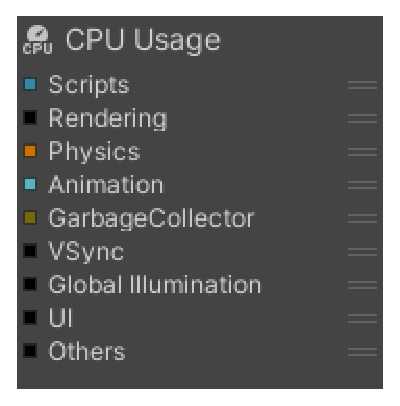
\includegraphics[width=0.5\textwidth]{grafika/profiler_settings.eps}
    \caption{Usage categories selected when analyzing CPU usage}
    \label{fig:profiler_settings}
\end{figure}

Starting with the baked version of the spider, a hundred duplicates spawned
simultaneously produced the result seen in Fig. \ref{fig:pr_sp_b}. Similarly
to the IK version presented further down, most of the CPU usage comes from the
"scripts" usage category. A clear distinction can be made between when the
spider was moving and when it was not. During the profiling, the state of the
spider started out as idle, and then alternated between moving and idle at
approximately each quarter of the graph presented. In the idle state, the CPU
usage for the selected categories remains steadily below 10 milliseconds.
However, when the spider is moving the usage rises with an initial spike which
is almost double that of the idle state, and then lowering to around 10
milliseconds. The increase in CPU usage, as seen from the profiler, is mostly in
the "scripts" category, which means that the animations themselves are not
influencing the performance of the application too much.

\begin{figure}[h!]
    \centering
    \captionsetup{justification=centering}
    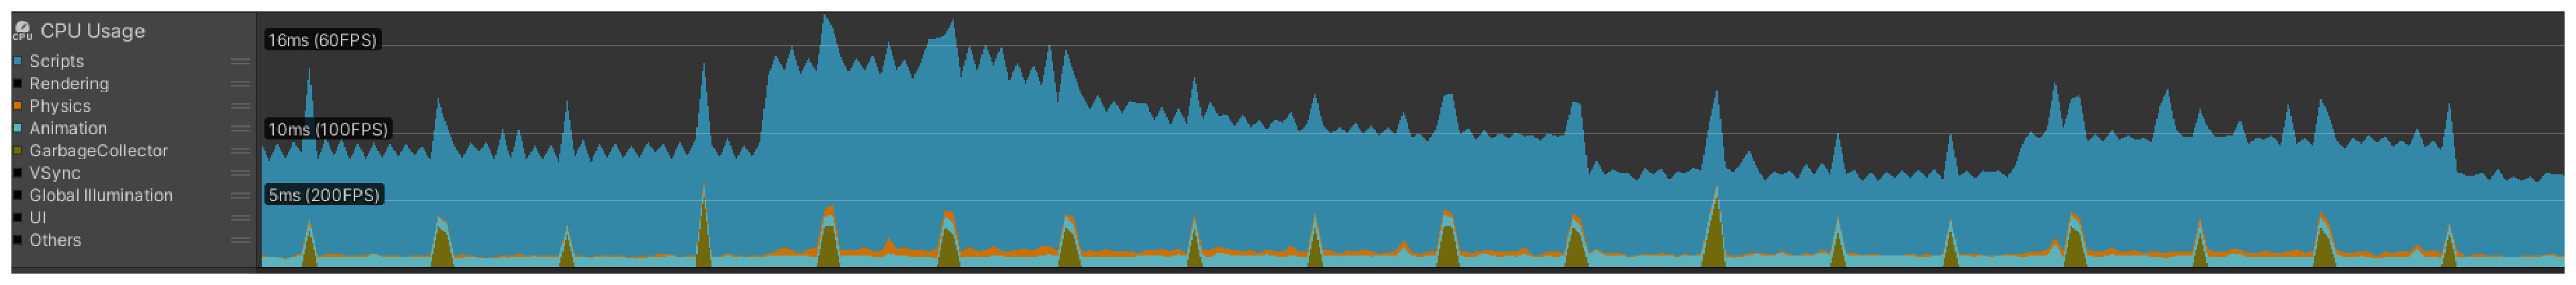
\includegraphics[width=\textwidth]{grafika/pr_sp_b.eps}
    \caption{Profiling of a hundred instances of the baked animation spider for
    CPU usage}
    \label{fig:pr_sp_b}
\end{figure}

The IK version of the spider has a much more steady average regardless of its
moving or idle state. In Fig. \ref{fig:pr_sp_ik}, the graph rises minimally at the
halfway mark which is where the spiders were transitioned to a moving state.
The lack of distinct change between states can be attributed to the fact that
the IK calculations done on the kinematic chains and their respective targets
are done regardless if the spider is moving or not. The same can be said for the
raycasts and body rotation calculations which are executed no matter the state.
The slight increase is most likely due to the calculations required to determine
the forward movement vector when the spider receives input. 

\begin{figure}[h!]
    \centering
    \captionsetup{justification=centering}
    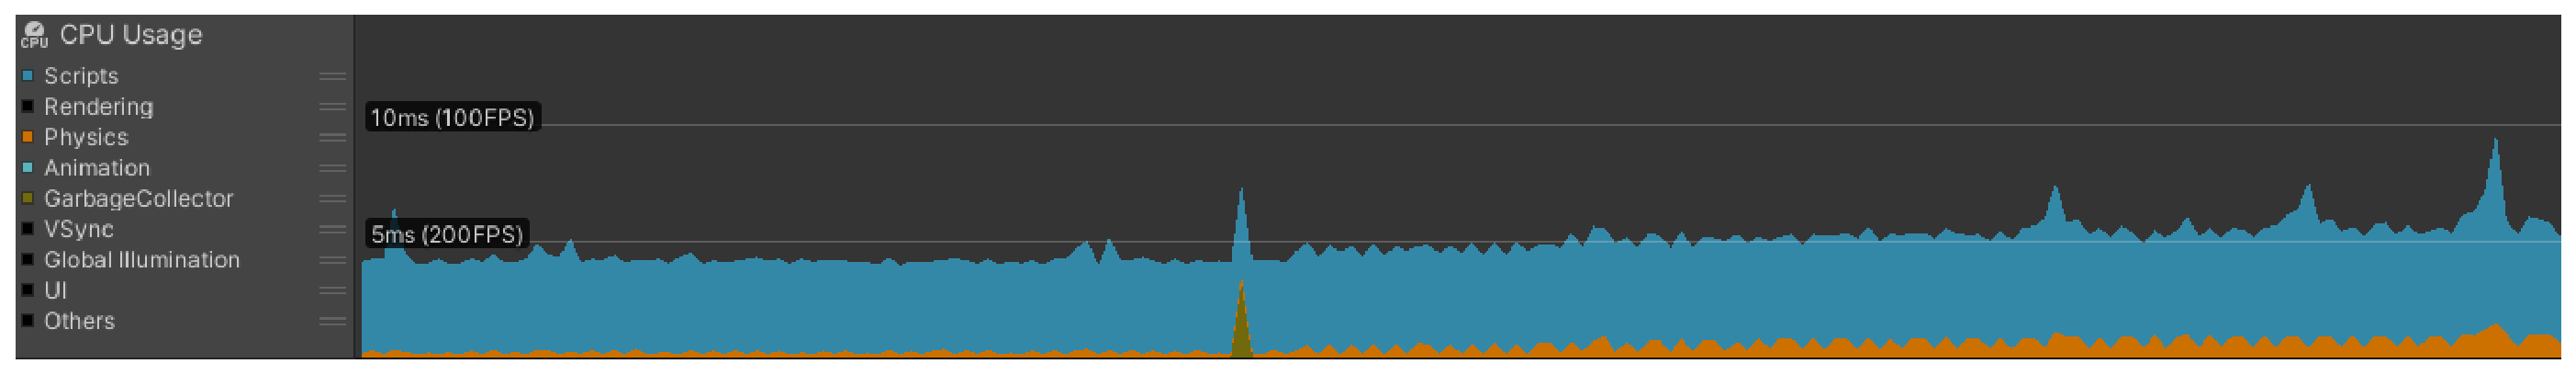
\includegraphics[width=\textwidth]{grafika/pr_sp_ik.eps}
    \caption{Profiling of a hundred instances of the procedurally animated
    spider for CPU usage}
    \label{fig:pr_sp_ik}
\end{figure}

The average CPU usage for the IK version of the spider is around half that of its
baked counterpart. This is most likely due to the baked animation spider
requiring more checks and calculations which pertain to the physics of its
movement. The IK version does not need many physics checks as the simple ray
cast system keeps the spider stuck to the surface, and combined with the IK
mechanism it moves the spider along without the need for collision checking.
However, this is relevant for the implementation presented in this demo
application, and may not be the case if a given use case required the spider to
be able to register collisions and be affected by gravity.

The purpose of the human character in the demo application is to demonstrate
a specific animation sequence executed through the means of baked and procedural
animations. Because there are no collisions, movement, or other checks, the baked
animation character's script contains almost no major calculations. Since
baked animations do not have a big influence on the CPU usage as seen earlier in
the case of the spider, the performance of the application does not vary in
relation to when the button pressing sequence is executed. Fig.
\ref{fig:pr_h_b} displays the results of profiling one hundred instances of the
baked animation human characters executing the animation sequence
simultaneously, and no spike in CPU usage, which hovers around 1ms, can be
observed

\begin{figure}[h!]
    \centering
    \captionsetup{justification=centering}
    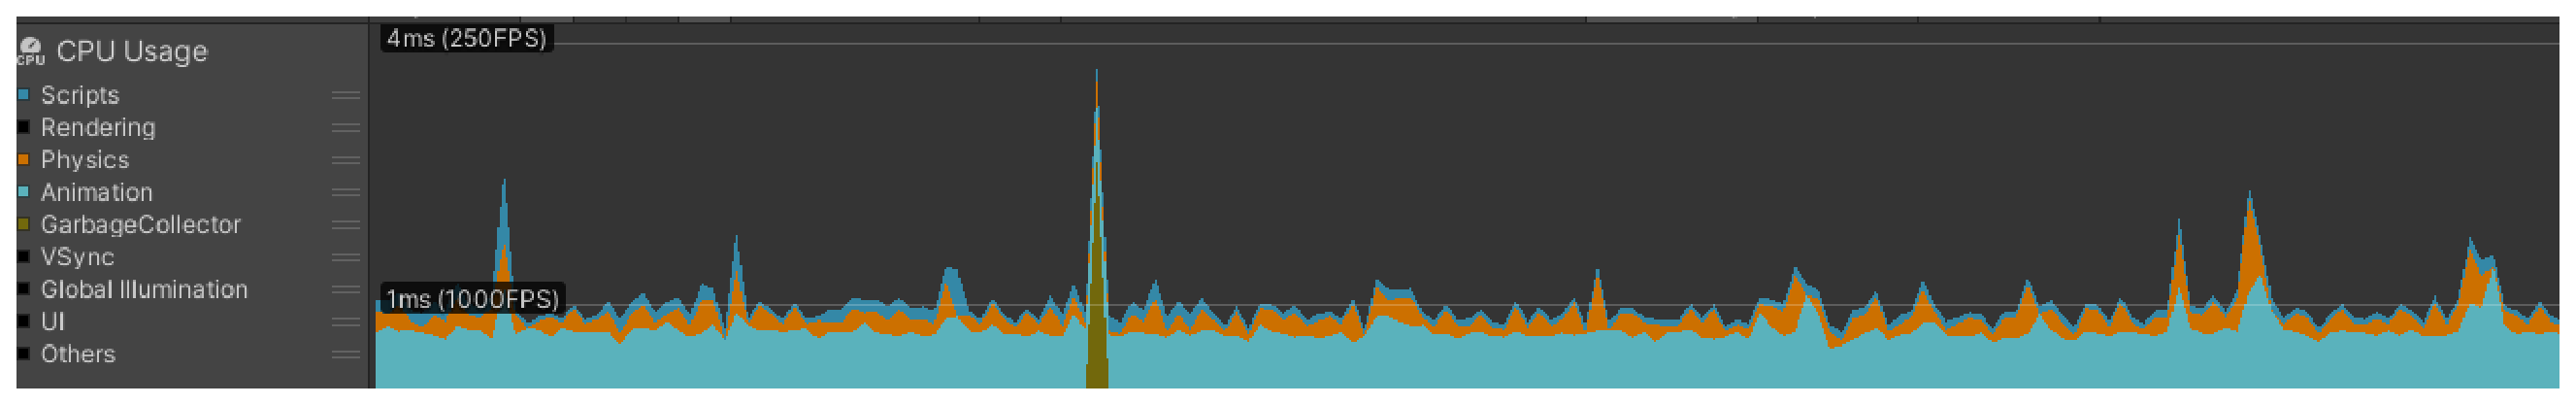
\includegraphics[width=\textwidth]{grafika/pr_h_b.eps}
    \caption{Profiling of a hundred instances of the human character with baked
    animations for CPU usage}
    \label{fig:pr_h_b}
\end{figure}

In contrast, the procedurally animated human does require a few calculations
during the animations sequence. While it does use baked animations for the
beginning and end of the sequence, the middle section switches to using inverse
kinematics, and additionally the IK targets are interpolated between the hand's
origin position and the button target positions. These calculations can be
seen in Fig. \ref{fig:pr_h_ik} where during the execution of the animation
there is a noticeable spike in the "scripts" usage category. Other than that,
the rest of the graph looks very similar to the baked animation variant, sitting
at around 1 milliseconds of CPU usage.

\begin{figure}[h!]
    \centering
    \captionsetup{justification=centering}
    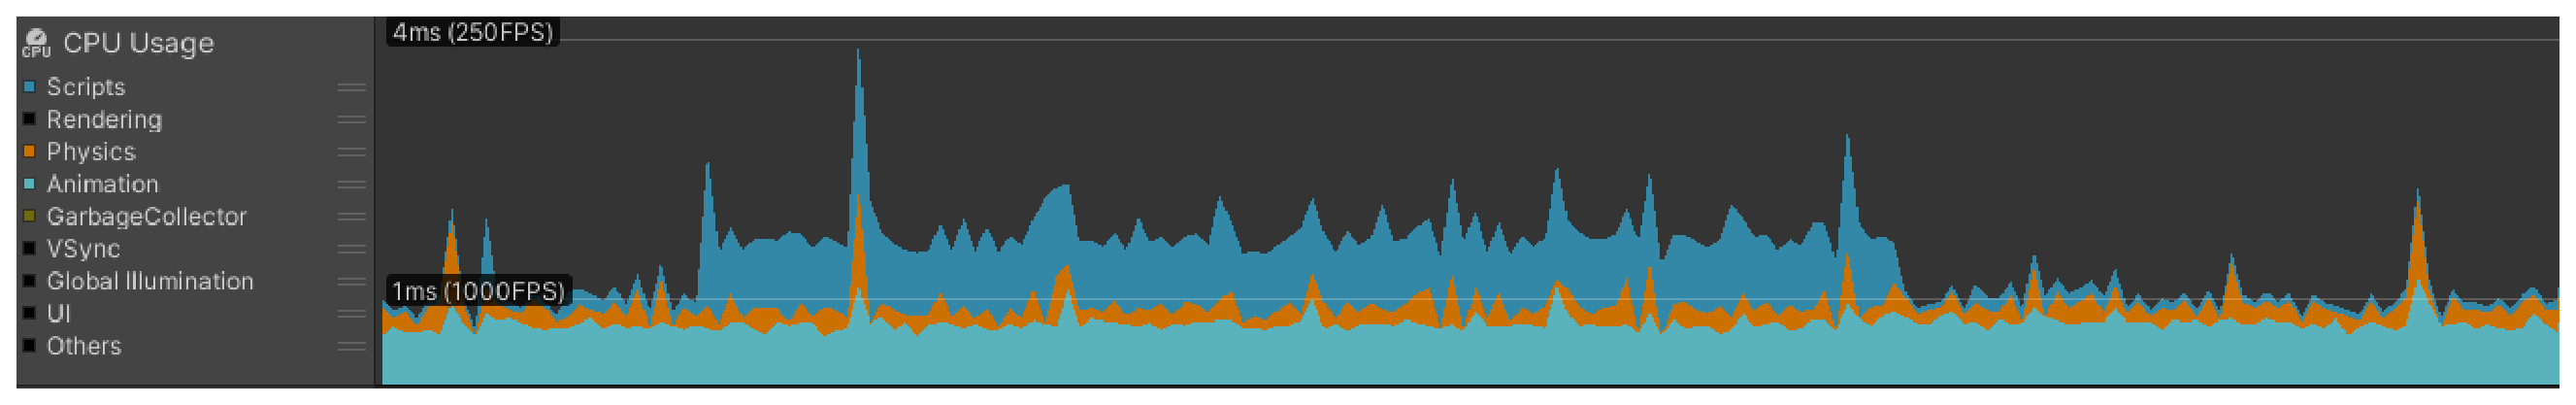
\includegraphics[width=\textwidth]{grafika/pr_h_ik.eps}
    \caption{Profiling of a hundred instances of the procedurally animated human
    for CPU usage}
    \label{fig:pr_h_ik}
\end{figure}



\chapter{Conclusion} 
The aim of this paper was to gain a better understanding of the basic algorithms
used in inverse kinematics, to discover the built-in functionalities that the Unity
engine offers for such implementation, and compare the IK procedural animations
to a classic baked animation approach through visual and performance based
metrics. The aim was achieved. 

In the second chapter, the theory behind existing IK
algorithms was analyzed. As a result of this analysis, the heuristic FABRIK
algorithm was chosen for its speed and simple implementation which distinguishes
itself from other approaches by avoiding problems such as instabilities and
complex calculations.

In the third chapter, an overview was made of technologies used in the
implementation of the demo application. Among others, the features provided by
the Unity game engine which enable and facilitate the use of IK were outlined.

The third and fourth chapters served to display the implementation details of
both the IK solutions and their baked animation counterparts, as well as compare
them in the visual and performance categories. In terms of visual realism and
natural motion, the IK animations proved to be superior in terms of precise
interaction with the surrounding environment, and the adaptability of the
characters to various situations. The human animation sequence demonstrated that
the procedural animations using inverse kinematics result in a higher CPU usage
compared to baked animations. However, the spider movement animation countered
this by showing that in certain cases, the procedural approach to animation and
movement can eliminate the need for various calculations such as physics checks,
and can overall result in a lower net CPU usage compared to a character which
has baked animations.



% \nocite{*} %wszystkie wpisy w bibliografi
\bibliographystyle{IEEEtranS} %{latex8} posortowane wzgledem wystepowania
\urlstyle{same}
\bibliography{bibliografia}%

\listoffigures
\listoftables
\lstlistoflistings


\end{document}
